\documentclass[a4paper]{article}

\usepackage{microtype}
\usepackage{fullpage}
\usepackage{setspace}
\usepackage{amsmath}
\usepackage{hyperref}
\usepackage{graphicx}
\usepackage{amsthm}
\usepackage{amssymb} 
\usepackage{booktabs}
\usepackage[labelsep=period]{caption}
\usepackage{subcaption}
\usepackage[noabbrev,nameinlink]{cleveref}
\usepackage[section]{placeins}
\usepackage{listings}
\usepackage{snapshot}
\usepackage{apptools}
\usepackage[backend=biber,style=authoryear,maxbibnames=99,hyperref=true]{biblatex}
\usepackage{mfirstuc}

\setstretch{1.15}

\hypersetup{colorlinks, citecolor=blue, filecolor=blue, linkcolor=blue, urlcolor=blue}

\addbibresource{src/paper/references.bib}
\DeclareFieldFormat{jtnoformat}{\capitalisewords{#1}}

\newcommand*{\latestversion}{\normalsize{Latest version: \href{https://stanmart.github.io/phd-thesis/experiment.pdf}{stanmart.github.io/phd-thesis/experiment.pdf}}}

\DeclareMathOperator*{\argmax}{argmax}

\newtheorem{proposition}{Proposition}

\AtAppendix{\counterwithin{proposition}{section}}
\AtAppendix{\counterwithin{equation}{section}}
\AtAppendix{\counterwithin{figure}{section}}
\AtAppendix{\counterwithin{table}{section}}

\lstset{
    basicstyle=\footnotesize\ttfamily,
    columns=flexible,
    breaklines=true,
}


\title{
    Characterizing Multiplayer Free-Form Bargaining: A Lab experiment%
    \thanks{
        We would like to thank our advisors, Nick Netzer, Marek Pycia, Armin Schmutzler, and Jakub Steiner for their invaluable feedback and support throughout this project.
        We are also grateful to Sandro Ambühl and Roberto A. Weber for the thoughtful suggestions about the design of the experiment.
        Finally, we thank the participants of the Behavioral Lab Meetings and the Market Design Seminar for their questions and comments.
    }
}

\author{
    Mia Lu\thanks{University of Zurich, mia.lu@econ.uzh.ch} 
    \and 
    Martin Stancsics\thanks{University of Zurich, martin.stancsics@econ.uzh.ch}
}

\date{July 30, 2024 \\\vspace{0.4cm} \latestversion}

\begin{document}

\maketitle

\begin{abstract}
    This experiment investigates coalition-formation and surplus division between three players in a free-form bargaining environment.
    We find that players' payoffs are increasing in their bargaining power, but only when forming a smaller coalition and excluding one of the non-monopolist players is a credible threat.
    This is qualitatively consistent with the theoretical predictions of the nucleolus from cooperative game theory, but the observed payoff inequality is significantly lower than the theoretical predictions.
    Our results highlight that fairness considerations seem to play an important role even under free-form bargaining: equal splits make up a large fraction of the outcomes, and fairness-related arguments are used frequently during bargaining.
    We also find considerable heterogeneity between players both in terms of bargaining behavior and stated preferences.
\end{abstract}

\section{Introduction} \label{sec:intro}

% general motivation  

Bargaining over how to share jointly produced surplus between parties of different bargaining power is ubiquitous - examples include wage bargaining, coalition discussions over the allocation of ministries between political parties, or bargaining over profits in a partnership. 
Consider for example an inventor who is in discussion with multiple investors for developing a new product. She can bring more than one investor on board and having multiple investors results in better product quality. How many investors will she bring on board and how will they split the profits? How much does this depend on the inventor's bargaining power?
%These are the type of questions we are interested in.  

The questions of coalition formation and payoff allocation have been studied extensively in the bargaining literature. However, only a small subset of papers studies bargaining behavior empirically. Moreover, bargaining in empirical tests is typically restricted to proposing or accepting coalitions and payoff allocations, even when unstructured. (``Unstructured bargaining'' typically refers only to no structure being imposed on the order or number of proposals, and does not allow for communication outside of numerical proposals.) In contrast to this, we study \emph{free-form} bargaining in our experiment where bargaining takes place via chat, without any restrictions. We believe this approach is much more realistic and captures relevant aspects of real-world bargaining, such as persuasion and explicitly expressed intention for example.

Furthermore, we are interested in how well solution concepts from cooperative game theory describe the bargaining outcomes in this setting. In particular, we focus on two of the most used and single-valued solution concepts: the Shapley value and the nucleolus. Both have suggestive experimental evidence \parencite{MurnighanRoth1977, MichenerPotter1981, ClippelRozen2022, KomoritaHamiltonKravitz1984, LeopoldWildburger1992} as well as theoretical backing in the sense that they can also be derived as solutions in extensive-form bargaining games \parencite{gul1989bargaining,hart1996bargaining,stole1996organizational}.

We focus on cooperative game theory for two main reasons. First, it is a natural choice for this setting with free-form bargaining and coalition formation.\footnote{Note that standard concepts from non-cooperative game theory are not applicable here as the action and strategy space are not well-defined in the free-form bargaining setting.} Second, the solution concepts we test are partly normative, and incorporate fairness notions.\footnote{The nucleolus reflects a mix of a Rawlsian notion of fairness and stability-based reasoning, while the Shapley value captures fairness in the sense of everybody getting their average marginal contribution.} One of the main conclusions of the extensive empirical literature on bargaining is that fairness considerations play a key role in determining the outcomes. Therefore, we might expect that these concepts do a reasonably good job of predicting the outcomes, even without explicitly relying on other-regarding preferences.

In our experiment, we study asymmetric bargaining between three players, where one player (the ``big player'') is a monopolist and without whom no value can be created. The other two players (the ``small players'') are symmetric to each other. No player can create any value on their own and the grand coalition creates more value than a small coalition between the big and a small player. We study this setting as we believe that this type of structure is representative of many real-world settings and because the effects of bargaining power are presumably more pronounced when the asymmetry is stronger. Players have five minutes to bargain over chat. Player roles are reassigned randomly every round, where a better performance in a slider task at the beginning of the experiment leads to a higher chance of becoming the big player. Subjects also fill out a survey where they indicate how much they agree with the characterizing axioms of the Shapley value and the stability property of the core. Our three main treatments vary the big player's bargaining power by varying how much value a small coalition between the big player and a small player creates. In a fourth treatment we test the dummy player axiom of the Shapley value which states that a dummy player that does not add any value to any coalition should receive zero.


We are interested in the following questions: First, how does the big player's bargaining power (as measured by the value of the small coalition, and thus the necessity of having both small players in the coalition) affect outcomes in multiplayer free-form bargaining. Second, how well is this captured by the Shapley value and the nucleolus? Finally, given our rich data (chat data, timing of proposals and acceptances, survey questions), how can we characterize the outcomes and bargaining behavior in general in this setting?

% what we do in this paper


% what we find


% results: main result, CGT fit and outcomes in general
We find that bargaining power is indeed reflected in the bargaining outcomes: the big player's share is increasing in their bargaining power. While none of the two cooperative game theory concepts are a good fit quantitatively, the nucleolus' qualitative predictions are correct. Interestingly, high payoffs for the big player are only realized by excluding one of the small players. Our results also highlight that fairness considerations seem to play an important role, even in this quite asymmetric setting, where bargaining positions are additionally ``earned'' to a certain degree: As much of the literature, we observe a large fraction of equal splits and even players who add nothing to the coalition's value receive a fifth of the grand coalition's worth on average. This implies that despite their fairness-based intuition, the solution concepts we test do not capture all aspects of players' fairness considerations.

% results: axioms
In terms of characterizing axioms, we find moderate support for the efficiency and symmetry axioms, and moderate to strong support against the dummy player, linearity and stability axioms. Additionally, subjects' stated preferences in the survey are not always consistent with observed outcomes. Especially in the case of the linearity and the stability axioms, stated preferences and observed outcomes differ.


% results: bargaining process
Regarding the bargaining process, we find that subjects often agree on an allocation very early in the negotiation phase, especially in the lower-bargaining-power treatments. In the higher-bargaining-power treatment, however, agreements are made later on average. This is in line with the high-bargaining-power treatment being associated with more intense bargaining. Furthermore, we find that within bargaining-related messages, the use of fairness-related arguments is relatively frequent, especially in the treatments with higher bargaining power disparity. 
%  chat

% structure of the paper

The rest of the paper is organized as follows. \Cref{sec:literature} provides an overview of the relevant literature. In \Cref{sec:theory}, we describe the coalitional game we use in the bargaining and discuss the theoretical predictions of the Shapley value and the nucleolus. \Cref{sec:exp_design} details the experimental design. In \Cref{sec:analysis}, we present the main results as well as the exploratory analysis of the bargaining process. \Cref{sec:conclusion} concludes.


%%%%%%%%%%%%%%%%%%%%%%%%%%%%%%%%%%%%%%%%%%%%%%%%%%%%%%%%%%%%%

\section{Related literature} \label{sec:literature}
This paper contributes to the large literature on bargaining by studying free-form bargaining via chat between more than two players. We analyze the bargaining outcomes and the process leading up to them, and test the fit of common models and axioms from cooperative game theory. Our paper is related to three different strands of the experimental bargaining literature: (1) unstructured multi-player-bargaining,\footnote{With ``unstructured bargaining'', we refer to any bargaining game where the number and order of proposals and acceptances is unrestricted. This does not necessarily entail additional means of communication.} (2) free-form bargaining\footnote{By ``free-form bargaining'', we mean that communication between players is unrestricted in terms of the content of their messages.} via chat and (3) fairness in bargaining. 

% early papers

\paragraph{Unstructured multi-player bargaining.}

Unstructured bargaining games with more than two players have been studied extensively in experimental economics \parencite[e.g.][]{Kalischetal1952, Maschler1965, NydeggerOwen1974, RapoportKahan1976, MurnighanRoth1978, Micheneretal1979, RothMalouf1979, KomoritaHamiltonKravitz1984, LeopoldWildburger1992}. The early literature\footnote{See \cite{Roth1995} for a review.} focused mostly on testing the fit of popular cooperative game theory concepts (such as the Shapley value, the Nash bargaining solution, kernel or nucleolus), and varied greatly in terms of which concepts they found support for. In recent years there has been a resurgence of unstructured bargaining experiments,\footnote{See \cite{karagozouglu2019going} for a review.} moving away from testing theoretic models to studying specific empirical relationships such as how uncertain information about performance affects subjective entitlement and subsequent bargaining \parencite{KaragözoğluRiedl2015}, the effect of payoff-irrelevant framing \parencite{Isonietal2014}, or the dynamics of coalition formation \parencite{TremewanVanberg2016}.

In this strand of literature, bargaining is typically still quite restricted. Communication is typically limited to sending acceptances or numerical proposals and verbal communication is not possible or very limited (for example, at most one verbal message per numerical proposal).\footnote{While some free-form bargaining was studied in the early papers, it always took the form of face-to-face bargaining. \textcite{LeopoldWildburger1992}, which utilizes three-player coalitional face-to-face bargaining, is closely related to our paper. We study a similar setting but are interested in free-form bargaining via chat instead of face-to-face. This allows us to abstract from factors such as loss of anonymity or appearance, while keeping the free-form and more natural character of face-to-face bargaining.} We contribute to this literature by allowing for completely unrestricted written communication, thus allowing for much more realistic bargaining. 

Most closely related to our paper is \textcite{MurnighanRoth1977}, which features an extreme version of our three-player game. One of the players is a monopolist that is needed to create value, while the two other players are completely substitutable. They study the effect of information and communication in unstructured bargaining by varying whether payoff divisions, messages and offers are secret or announced. They find that the results closely approximate the Shapley value, while we find much less support for the Shapley value in our experiment. This is consistent with their finding that more communication leads to smaller monopolist payoffs, as communication is much more unrestricted in our case. Additionally, in their case the grand coalition created the same value as the small coalition. In our study, the grand coalition was (often much) more attractive than the small coalition, which might explain why we observe much more grand coalitions and outcomes closer to the equal split.


\paragraph{Free-form bargaining via chat.}

Several papers have gone beyond unstructured bargaining and used free-form bargaining via chat \parencite{LuhanPoulsenRoos2019, Galeottietal2018, HossainLyonsSiow2020, NavarroVeszteg2020, ShinodaFunaki2022, Schwaninger2022, Takeuchietal2022}. They typically find that fairness considerations play an important role and can lead to inefficiencies. Furthermore, fairness concerns seem to be heavily context dependent, e.g. they can vary significantly with slight changes of the functional form of the production function \parencite[]{Takeuchietal2022} or with the framing as a partnership as opposed to an employment relationship \parencite{HossainLyonsSiow2020}.

Almost all of these free-form papers focus on bilateral bargaining. Our paper contributes to this literature by studying three-player settings which allow us to study coalitional behavior and provides a richer environment for studying how varying the bargaining power between players affects bargaining outcomes. Furthermore, it also allows for testing cooperative solution concepts, which are less relevant in the two-player case.

Most closely related to our paper, \textcite{ShinodaFunaki2022} study how the existence of the core affects bargaining outcomes and also have treatments with a public chat in a three-player coalitional bargaining setting. However, in their study ``subjects sent very few messages through the chat window. [...] One possible reason is that the subjects were too busy making offers and reacting to others' offers to send messages.'' In our study, the chat plays a central role and subjects actively used the chat to negotiate. Apart from a substantially different research question, this paper also differs from \textcite{ShinodaFunaki2022} by studying the bargaining process in detail and the empirical support of common cooperative game theory axioms.


\paragraph{Fairness in bargaining.}

More broadly, we contribute to the vast literature on fairness in bargaining, which was started by the seminal paper of \textcite{Güthetal1982} and has focused on structured two-player games (primarily variations of the ultimatum bargaining game). The main insight is that, contrary to standard game-theoretical predictions, fairness matters also in a structured bargaining game and subjects care about other players' payoffs: in the ultimatum game proposers offer about 40 percent on average, while responders often reject offers under 20 percent. However, subjects are not necessarily primarily trying to be fair \parencite[]{Roth1995}, and there is also considerable evidence that fairness concerns are not stable, in the sense that they are easily influenced by small changes of the game, often leading to results much closer to standard theoretical predictions \parencite[e.g.]{Binmoreetal1985, GrimmMengel2011}. We add to this literature by studying settings that add more realism; i) by allowing free-form communication and ii) by using a coalitional setting where players' contributions to the value to be distributed are less clear-cut. Nevertheless, we find support for the same stylized fact: outcomes are much closer to equal split than what (cooperative or non-cooperative) game theoretical models would predict.

% fairness preferences papers (subjects as impartial spectators)
Another strand of this literature explicitly studies subjects' distributive preferences as impartial spectators, thus eliminating strategic concerns (for example \cite{cappelen2007pluralism, LuhanPoulsenRoos2019, AlmasCappelenTungodden2020, ClippelRozen2022}). \textcite{ClippelRozen2022} study classic cooperative game theory questions from a different perspective; they analyze how outside observers of a three-player coalitional game distribute the coalitional worth between players. They find that a convex combination of the Shapley value and the equal split offers a good description of the outcomes. This is in contrast to our results, which are more consistent with a mix of the equal split and the nucleolus.

%%%%%%%%%%%%%%%%%%%%%%%%%%%%%%%%%%%%%%%%%%%%%%%%%%%%%%%%%%%%%

\section{Theory} \label{sec:theory}

A \emph{cooperative (or coalitional) game} $\mathcal{G}$ is defined by the set of players $N$, and the characteristic (or value) function $v: 2^N \to \mathbb{R}^{|N|}$:
\begin{align*}
    \mathcal{G} = (N, v).
\end{align*}
The main difference compared to non-cooperative game theory (NCGT) is that the structure of the game is specified in less detail. Instead of describing the action space and the corresponding strategy space, cooperative game theory (CGT) takes a more reduced-form approach: one only needs to characterize the value each subset of players ($S \subset N$) can generate ($v(S)$), but how they do so is not important. On one hand, it makes CGT blind to certain, perhaps important attributes of a game.\footnote{An example of this would be who the proposer is in an ultimatum game.} On the other hand, this means that CGT is suitable to describe situations where the exact strategy space is not known. An example of the latter is the bargaining game presented in this paper. Due to the free-form nature of the bargaining, the order of actions is not well-defined.\footnote{In the realm of non-cooperative games, such situations are often modeled with some kind of alternating offer games \parencite[e.g.][]{rubinstein1982perfect,gul1989bargaining}. However, as \textcite{hart1996bargaining} demonstrates, the equilibrium in these games can be rather sensitive to small changes in assumptions.}

\subsection{Solution concepts}

Much of cooperative game theory has traditionally focused on the study of superadditive (also known as proper) games. Superadditivity is a property that ensures that any two disjoint coalitions are weakly better off by merging.\footnote{Formally, for any $S_1, S_2 \subset N$ with $S_1 \cap S_2 = \emptyset$, $v(S_1) + v(S_2) \leq v(S_1 \cup S_2)$.} As a consequence, it is rational for the grand coalition (i.e., the coalition of every player) to form. Subsequently, solution concepts aim to describe how the value generated by the grand coalition, $v(N)$, should be divided across its members.

One trivial, but nevertheless important way to divide the total value is the \emph{equal split}. That is, each player gets an equal share of the grand coalition's value: $\frac{v(N)}{|N|}$. It's predictions do not depend on the value function (apart from the value of the grand coalition), and are thus blind to how players differ in terms of their contributions and bargaining positions. Nevertheless, one might expect it to be a somewhat frequent bargaining outcome for two reasons. First, it embodies an extremely natural fairness concept which is easy to agree on. Second, it is a very salient allocation, and might serve as a focal point during bargaining.

Amongst the more usual cooperative solution concepts, arguably the two most commonly used ones are the core \parencite{gillies1959solutions} and the Shapley value \parencite{shapley1953value}. The core is based on stability notions, not unlike the Nash-equilibrium from non-cooperative game theory. Conversely, the Shapley value is based on the contribution of each player to the value, making it more fairness related. The next sections describe these two concepts in more detail, as well as the nucleolus, which is related to the core but possesses better properties and incorporates certain fairness considerations.

\subsubsection{Core} \label{stability_statement}

The core is the set of payoff vectors for which no coalition $S \subset N$ is better off by deviating and distributing $v(S)$ among themselves. In this respect, it is similar to the Nash equilibrium, but instead of just unilateral deviations, it takes multi-player deviations into account.

In order to characterize the core formally, let us first define the concept of the \emph{excess}. Let $x \in \mathbb{R}^{|N|}$ be a payoff vector that is efficient and individually rational (also known as an imputation).\footnote{The set of imputations $X$ is defined by $x \in X$ iff $x$ satisfies $\sum_{i \in N} x_i = v(N)$ and $x_i \geq v(\{i\})$ for all $i \in N$.} The excess of $x$ for a coalition $S$ is the difference between the total payoff of its members and the value they could get on their own:
\begin{align*}
    e(x, S) = \sum_{i \in S} x_i - v(S).
\end{align*}
The \emph{core} is defined as the set of imputations for which the excess is non-negative:
\begin{align*}
    c(v) = \{x \in X \mid e(x, S) \geq 0 \;\forall\, S \subset N\}
\end{align*}
This is equivalent to no coalition having an incentive to deviate, as the coalition members can not achieve a higher payoff on their own.

While the core is appealing on account of its simple, stability-based definition, it has a number of troublesome properties. For one, existence is not guaranteed: the core can be empty. Furthermore, uniqueness is also not guaranteed, and the core is often multi-valued. These attributes restrict its usefulness as a predictive tool.

\subsubsection{Nucleolus}

The \emph{nucleolus} \parencite{schmeidler1969nucleolus} is an attempt to guarantee existence and uniqueness, while at the same time not deviating too far from the stability-based idea behind the core. It can be defined as the allocation that maximizes the smallest excess across all coalitions:\footnote{Technically, this is not the complete definition, as it does not always guarantee uniqueness. \textcite{schmeidler1969nucleolus} also prescribes that if multiple imputations maximize this expression, then the second smallest excess is maximized, and so on in a lexicographic manner. However, due to no such ties occurring in our game, we ignore this detail to simplify exposition.}
\begin{align*}
    n(v) = \argmax_{x \in X} \min_{S \subset N} e(x, S).
\end{align*}

\textcite{schmeidler1969nucleolus} motivates this definition with the argument that, for any given allocation, the coalition that is expected to object most strongly to it is the one with the lowest excess. In this sense, the nucleolus combines a Rawlsian fairness argument with the stability-based definition of the core. Another justification for the nucleolus is its relation to the core: if the latter is non-empty, then it contains the nucleolus.\footnote{This observation immediately follows from the excess-based definition of the two solution concepts. If there is an imputation where all excesses are non-negative, then the one maximizing the minimum excess will also satisfy this property.} It thus shares the stability-based definition with the core, while being unique, and thus more suitable for empirical analysis.

\subsubsection{Shapley value}

The \emph{Shapley value} \parencite{shapley1953value} takes a wholly different approach in comparison to the previous two solution concepts. Instead of relying on stability-related notions, it allocates the payoffs based on the marginal contributions of the players. Therefore, it can be considered as a fairness-based solution concept.

According to the Shapley value, each player should get their average marginal contribution to the value of the grand coalition, where the average is taken over all orderings of players. Formally, let $R$ be a permutation of $N$. Let us denote the players preceding $i$ in permutation $R$ as $\mathcal{P}_i^R$. Then, the Shapley value of player $i$, $\varphi_i$, is defined as follows:
\begin{align}
    \varphi_i(v) = \frac{1}{|N|!}\sum_R \left[ v(\mathcal{P}_i^R \cup \{i\})  - v(\mathcal{P}_i^R) \right]. \label{eq:shapley_vale}
\end{align}
Due to having a closed-form definition, it is immediate that the Shapley value always exists and is unique.

In addition to this marginal-contribution-based definition, the Shapley value also has a number of axiomatic characterizations. The most well-known one is due to \textcite{shapley1953value}, and states that the Shapley value is the unique allocation that satisfies the following four axioms.
\begin{description}
    \item[Efficiency] The full value of the grand coalition is distributed: $\sum_{i \in N} \varphi_i(v) = v(N)$.
    \item[Symmetry] Any two players who are equivalent in terms of the value function get the same amount. I.e., if $v(S \cup \{i\}) = v(S \cup \{j\}) \;\forall\, S \in N \setminus \{i, j\}$, then $\varphi_i(v) = \varphi_j(v)$.
    \item[Null player axiom] A player whose marginal contribution to any coalition is zero gets nothing. Formally, if for some $i$, $v(S \cup \{i\} = v(S) \;\forall\, S$, then $\varphi_i(v) = 0$.
    \item[Linearity] If two games with the same set of players are combined such that the new value function is a linear combination of the original ones, then the outcome for each player is a also linear combination of their previous outcomes, and with the same coefficients. Formally, let $\mathcal{G}_1 = (N, v)$ and $\mathcal{G}_2 = (N, w)$. Then, $\varphi(\alpha v + \beta w) = \alpha \varphi(v) + \beta \varphi(w)$, for any $\alpha, \beta \in \mathbb{R}$.
\end{description} \label{axioms_statement}

The first two axioms are rather straightforward and make intuitive sense from a fairness point of view. On the other hand, the null player axiom is more questionable. The latter can be violated, for example, due to altruism or social norms. Famously, a number of experiments \parencite[for a meta-analysis, see][]{engel2011dictator} demonstrate that proposers are generally willing to give some money to the other player in dictator games, even though the latter does not have any effect on the payoffs. Finally, the linearity axiom is arguably the main defining property of the Shapley value. Its relation to fairness, while less evident, follows from the fact that any value that is a weighted combination of the marginal contributions must satisfy this property \parencite{weber1988probabilistic}.\footnote{Besides the marginal-contribution-based interpretation and the axiomatic characterization, there is a series of papers that provide non-cooperative microfoundations for the Shapley value, providing another justification for using it in bargaining-related settings. Most models in this strand of literature \parencite[e.g.][]{hart1996bargaining,gul1989bargaining,stole1996organizational} rely on extensive form alternating offer games, of which the Shapley value is a subgame perfect equilibrium. Such results also exist for other types of games, such as demand commitment games \parencite{winter1994demand} or auctions \parencite{van2021allocating}.}


\subsection{The games in the experiment}

Let us now formally define the played in this experiment in coalitional form. They can be classified into two categories: the main treatments and the dummy player treatment. 

\subsubsection{Main treatments} \label{explanation_main_treatments}

There are three players in the game:
\begin{align*}
    N = \{A, B_1, B_2\}.
\end{align*}
We call $A$ the ``big player'', and refer to the other two as ``small players''. The value any subset of them creates is described by the following characteristic function:
\begin{align*}
    v_Y(S) = \begin{cases}
        100 & \text{if}\ S = \{A, B_1, B_2\} \\
        Y & \text{if}\ S = \{A, B_1\} \text{ or } S = \{A, B_2\} \\
        0 & \text{otherwise}
    \end{cases}
\end{align*}
with $Y \in (0, 100)$. Let us define the game $\mathcal{G}_Y = (N, v_Y)$.

In this game, Player $A$ must be included in the coalition to create any value, whereas Players $B_1$ and $B_2$ are not indispensable. At least one of the small players is also required, and both are needed to get the maximum of $100$, but even one of them is sufficient to create some amount of value $Y \in [0, 100]$. On an intuitive level, this implies that in a bargaining situation, the big player has more bargaining power than the small ones (hence the names). Furthermore, one could argue that this bargaining power advantage is increasing in $Y$: When $Y$ is higher, having both small players on board is less important, as a larger fraction of the total value can be achieved with just one of them being in the coalition. This might give Player $A$ more leeway to negotiate against the small players, or even play them against each other.

Let us now verify if the solution concepts described in the previous section agree with this intuition. We focus on the nucleolus and the Shapley value due to them being unique.\footnote{It can also be shown that the core is also increasing in $Y$, in the sense that the allocation in the core in which Player $A$ gets the lowest amount increases as $Y$ becomes larger.} The following propositions establish their predictions for this particular game.

\begin{proposition}
    \label{prop:shapley_value}
    Let $\varphi_i(v_Y)$ denote the Shapley value of player $i \in \{A, B_1, B_2\}$ in the game $\mathcal{G}_Y$. Then,
    \begin{align*}
        \varphi_A(v_Y) &= \frac{100}{3} + \frac{Y}{3}, \\
        \varphi_{B_i}(v_Y) &= \frac{100}{3} - \frac{Y}{6}.
    \end{align*}
\end{proposition}
\begin{proof}
    Simply substitute $v_Y$ into \Cref{eq:shapley_vale} to obtain
    \begin{align*}
        \varphi_A(v_Y) &= \frac{1}{6} \left[ 0+0+Y+Y+100+100 \right] = \frac{100}{3} + \frac{Y}{3}, \\
        \varphi_{B_i}(v_Y) &= \frac{1}{6} \left[ 0+0+0+Y+(100-Y)+(100-Y) \right] = \frac{100}{3} - \frac{Y}{6}.
    \end{align*}
\end{proof}

\begin{proposition}
    \label{prop:nucleolus}
    Let $n_i(v_Y)$ denote the element of the nucleolus corresponding to player $i \in \{A, B_1, B_2\}$ in the game $\mathcal{G}_Y$. Then,
    \begin{align*}
        n_A(v_Y) &= \begin{cases}
            \frac{100}{3} & \text{if}\ Y \leq \frac{100}{3} \\
            Y & \text{if}\ Y > \frac{100}{3}
        \end{cases}, \\
        n_{B_i}(v_Y) &= \begin{cases}
            \frac{100}{3} & \text{if}\ Y \leq \frac{100}{3} \\
            50 - \frac{Y}{2} & \text{if}\ Y > \frac{100}{3}
        \end{cases} 
    \end{align*}
\end{proposition}
\begin{proof}
    Due to the symmetry of the nucleolus \parencite{snijders1995axiomatization}, any nucleolus-candidate can be characterized by $x_A$ (the payoff of Player $A$). Furthermore, due to the fact that $e(\{B_i\}, x) \leq e(\{B_1, B_2\}, x) \;\forall\, x\in X$, we only have to consider the following three excesses when maximizing the smallest one:
    \begin{align}
        e(\{A\}, x) &= x_A, \label{eq:excess_A} \\
        e(\{B_i\}, x) &= \frac{100-x_A}{2}, \label{eq:excess_B} \\
        e(\{A, B_i\}, x) &= x_A + \frac{100-x_A}{2} - Y. \label{eq:excess_AB}
    \end{align}
    For $Y \leq \frac{100}{3}$, \Cref{eq:excess_B,eq:excess_A} are binding when $x_A$ is chosen to maximize the smallest one, and consequently, $x_A = \frac{100}{3}$. When $Y > \frac{100}{3}$, \Cref{eq:excess_B,eq:excess_AB} are the smallest, and thus $x_A = Y$.
\end{proof}

\begin{figure}
    \centering
    \includegraphics[width=.9\linewidth]{out/figures/values_theory.pdf}
    \caption{The Shapley value, the nucleolus and the equal split value for Player $A$ in the main game as a function of the value of the small coalition. The small players share the rest of the value equally. The dashed vertical lines denote the three main treatment arms in the experiment.}
    \label{fig:values_theory}
\end{figure}

\Cref{fig:values_theory} summarizes the content of \Cref{prop:nucleolus,prop:shapley_value} for Player $A$. It demonstrates that the studied solution concepts do agree with the intuitive expectations to some extent. The big player is always predicted to get at least much as the small ones, with the inequality always being strict for the Shapley value, and strict for high enough $Y$ for the nucleolus. Furthermore, the share of Player $A$ is indeed increasing in $Y$. This increase is always strict in the case of the Shapley value. For the nucleolus, this is not the case: it coincides with the equal split for $Y \leq \frac{100}{3}$, but then increases strictly (and much faster than the Shapley value) for the rest of the interval.

These differences can be understood by looking at the defining characteristics of these concepts. The Shapley value is based on marginal contributions. As the marginal contribution of $A$ to the coalitions $\{B_1\}$ and $\{B_2\}$ strictly increases in $Y$, its Shapley value will also strictly increase. Furthermore, as the marginal contributions of the small players are never zero, their Shapley values remain positive even as $Y \to 0$.

On the other hand, the nucleolus is related to the core, which is a stability-based concept. When $Y \leq \frac{100}{3}$, the big player does not have an actual bargaining edge over the small players, as no deviating player could gain more than what they get from the equal split. As a consequence, the nucleolus coincides with the equal split on this interval. However, when $Y > \frac{100}{3}$, the situation is different, and the difference in roles starts to play a role.\footnote{The equal split is still in the core for any $Y \leq \frac{200}{3}$. The nucleolus is just one particular element of the core, so this stability-based intuition only goes so far.} In particular, for high values of $Y$, Player $A$ possesses practically all the bargaining power, as forming a coalition with one of the small players and excluding the other becomes a credible threat.

\subsubsection{Dummy player treatment} \label{explanation_dummy_player_treatment}

The other game that is played in our experiment is somewhat different. There are still three players, but now let us call them $N_D = \{A_1, A_2, B\}$. $A_1$ and $A_2$ are referred to as the ``non-dummy-players'', while $B$ is the ``dummy player''. The characteristic function for the game $\mathcal{G}_D = (N_D, v_D)$ is defined as follows:
\begin{align*}
    v_Y(S) = \begin{cases}
        100 & \text{if}\ A_1, A_2 \in S \\
        0 & \text{otherwise}
    \end{cases}.
\end{align*}
In words, both of the non-dummy players are necessary to create any value, but the dummy player does not have any contribution at all (cf. the dummy player axiom).

As the next proposition shows, the Shapley value and the nucleolus agree on the predicted outcome in this game: the non-dummy players should share the total value equally, while the dummy player gets nothing.\footnote{The core is also single-valued for this game, and coincides with the other two solution concepts.}
\begin{proposition}
    \label{prop:dummy_player}
    The $\varphi(v_D)$ and $n(v_D)$ denote the vector of Shapley values and the nucleolus in the game $\mathcal{G}_D$. Then,
    \begin{align*}
        n_{A_i}(v_D) = \varphi_{A_i}(v_D) &= 50, \\
        n_{B}(v_D) = \varphi_{B}(v_D) &= 0.
    \end{align*}
\end{proposition}
\begin{proof}
    For the Shapley value, $\varphi_{B}(v_D)$ immediately follows from the dummy player axiom, and then $\varphi_{A_i}(v_D)$ is given by the symmetry axiom. In the case of the nucleolus, the excess for the coalition $\{A_1, A_2\}$ would be negative if $n_{B}(v_D) > 0$, while the minimum excess is 0 if $n_{B}(v_D) = 0$. Then $n_{A_i}(v_D) = 50$ can be obtained from the fact that the nucleolus also satisfies the symmetry axiom \parencite{snijders1995axiomatization}.
\end{proof}
In the case of the Shapley value, the reason for this is that the marginal contribution of the dummy player is zero to any coalition. For the nucleolus, the intuition is that if the dummy player were to get anything, then the two other players could deviate, form a coalition of their own, and share the total value.


%%%%%%%%%%%%%%%%%%%%%%%%%%%%%%%%%%%%%%%%%%%%%%%%%%%%%%%%%%%%%
\section{Experimental Design} \label{sec:exp_design}


% treatment
There were four experiment sessions in total. Each session corresponded to one of the four treatments: The three main treatments consisted of the game described in \Cref{explanation_main_treatments} and differed only in the value of the small coalition ($Y \in \{10,30,90\}$).\footnote{The values were chosen so as to allow for differentiation between the Shapley value and the nucleolus.} The fourth treatment was the dummy player treatment described in \Cref{explanation_dummy_player_treatment}. 

% session structure
Each experiment session was structured as follows: First, subjects went through the instructions, which included mandatory exercises, both as a comprehension check and so that participants could get used to the interface.\footnote{We refer to \Cref{subsec:instructions} for screenshots of the exact instructions and interface used in the experiment. Participants also received a printed-out version of the instructions as a reference during the experiment.} Subjects then played a version of the slider task \parencite{GillProwse2012slider}, which determined their role assignment later on. After a trial round, subjects played five bargaining rounds. At the end of the session, subjects filled out an exit survey and received their payment. 

Bargaining took place in a completely free-form manner via chat and an ancillary interface.\footnote{Refer to \Cref{sec:chat} for evidence that the chat was actually used for bargaining.} Each bargaining group had five minutes to decide on a coalition and a payoff allocation among coalition members. There was one public chat for each bargaining group.\footnote{Note that we do not allow for private communication. While private communication between bargainers is a feature of many real-world settings, we abstract from it here for simplicity. Our concern was that allowing for private communication could potentially overwhelm subjects who might have to monitor multiple text chats all at once.} Players' roles were also public in the chat, though their identity was anonymous.\footnote{However, some subjects discussed previous rounds' results in order to find out whether they had been rematched with the same subjects or even tried to establish code words.} 

To facilitate bargaining, subjects were given a bargaining interface.\footnote{See \Cref{bargaining_interface}. Past proposals were listed and given IDs for simpler reference during the bargaining in the chat.} Subjects could make an unlimited number of proposals. A proposal had to specify both the coalition and the payoff allocation. Only positive payoffs were allowed. Subjects could also indicate which proposal they currently accepted. They could change their acceptance decision any time and as often as they liked. The currently accepted decisions were then taken as the final decisions at the end of the bargaining round. A proposal was only successful if all coalition members agreed on the same proposal. The members of the successful coalition received their payoff according to the proposal, while the remaining player (if any) received nothing. As singleton coalitions had a value of 0, at most one proposal could be successful at a time. When no proposal was successful, all players received nothing. After each round, subjects were shown which coalition had formed and their resulting payoff.

At the end of the sessions and after learning their final payments, subjects filled out an exit survey. The survey asked for their agreement with the Shapley axioms and the defining property of the core (stability). We also collected basic demographic information (gender, age, study field, degree and nationality), as well as subjects' assessment of their own and others' strategies during the game.

% randomisation/ role and group assignment 

We used stranger matching in order to minimize reciprocity concerns. No set of subjects was matched twice (though individual players could be rematched). In order to account for dependence between rounds, in each session, the subjects were split into six matching groups (six subjects per matching group) and bargaining groups were only redrawn within a matching group. 

Players' roles varied across rounds and were reassigned at the beginning of each round, according to the slider task at the beginning: In each bargaining group, subjects were ranked in descending order with respect to how many sliders they had correctly moved. The role of the big player was assigned to the highest-ranking subject in the bargaining group with a probability of 0.5, to the second-ranking subject with a probability of 0.3 and to the lowest-ranking subject with a probability of 0.2.\footnote{Note that the slider task was designed so that subjects would not be able to finish it and that objectively evaluating their own performance would be very difficult for them. This was to ensure that subjects did not have any additional information about their slider task performance apart from their respective roles during the bargaining.} (In the dummy player treatment this was reversed: the dummy player role was assigned to the lowest-ranking subject with a probability of 0.5, and so on.) Note that subjects did not know about the exact probabilities, they were only told that a better (worse) performance led to a higher chance of becoming the big player (the dummy player). We believe that this increases realism in the sense that in the real world people usually only know that a given outcome is a result of effort and luck, but have no way of knowing the exact process with which the outcome was generated. Subjects were informed of their role in a given round right before the bargaining started.


The experiment was conducted in May 2024 at a computer lab at the University of Zurich and was written using oTree \parencite{CHEN201688}.\footnote{See \href{https://github.com/stanmart/unstructured-bargaining-experiment/releases/tag/main-experiment}{https://github.com/stanmart/unstructured-bargaining-experiment/releases/tag/main-experiment} for the full code (git commit hash: 64ae48773a3fcfff1d7af74e1c9b60d4082ddcd7), and \href{https://github.com/stanmart/unstructured-bargaining-experiment/releases/tag/main-experiment-fix-2}{https://github.com/stanmart/unstructured-bargaining-experiment/releases/tag/main-experiment-fix-2} for the version with a couple of minor fixes.}\footnote{The study was preregistered before data collection. The preregistration can be found at \href{https://www.socialscienceregistry.org/trials/13593}{https://www.socialscienceregistry.org/trials/13593}. Our analysis was conducted as specified there.} A total of 144 subjects participated in the experiment (36 subjects per treatment). There was no attrition during the sessions. Participants were recruited from the student bodies at the University of Zurich (UZH) and the Federal Institute of Technology Zurich (ETH).\footnote{For more information on characteristics of our sample, see \Cref{fig:balance}} Participants were only allowed to participate in one of the sessions. Sessions lasted about an hour. Participants bargained over experimental points (the grand coalition's payoff was 100 points). Payments constituted of a show-up payment of 10CHF and their average bargaining payoff in points across rounds, converted to CHF (with the conversion 1 point= 0.6CHF).\footnote{During the first session ($Y = 10$) we realized that the average payoffs were not displayed correctly after the bargaining rounds and used a corrected version of the experiment for the remaining sessions. We believe that this did not influence outcomes substantially  because this was only a matter of several points and the monotone relationship between bargaining payoffs in experimental points and the payment in CHF was untouched.} Subjects were paid in cash, and they earned about 30CHF on average. 
 



%%%%%%%%%%%%%%%%%%%%%%%%%%%%%%%%%%%%%%%%%%%%%%%%%%%%%%%%%%%%%
\section{Analysis} \label{sec:analysis}

\subsection{Main results}

Let us start by answering the main question of this paper: how does bargaining power, as measured by the necessity of having both small players in the coalition, impact bargaining outcomes? Remember that both the Shapley value and the nucleolus, as well as arguably most people's intuitions, predict that an increase in the bargaining power of the big player (i.e., a decrease in the necessity of having both small players included in the coalition) should lead to a decrease in the share of the small players. In terms of the experiment, it means that the share of the big player should be increasing in $Y$.

\begin{figure}
    \centering
    \includegraphics[width=.9\linewidth]{out/figures/payoff_average_rounds_all.pdf}
    \caption{Average payoffs for each player role by treatment. Vertical bars denote 95\% confidence intervals for the within-group means.}
    \label{fig:main_means}
\end{figure}

\Cref{fig:main_means} shows that this is indeed the case, for the most part.\footnote{The replication package for this paper can be obtained from  \\\href{https://github.com/stanmart/unstructured-bargaining-analysis/releases/tag/submitted}{https://github.com/stanmart/unstructured-bargaining-analysis/releases/tag/submitted}.} The average share of the big player in the $Y=90$ treatment is higher than in the other two treatments. However, the outcomes do not seem different between the $Y=10$ and $Y=30$ treatments. \Cref{tab:main_regressions} reinforces this observation. When included as a continuous variable, $Y$ is indeed positive and significant in the regression. For an increase in $Y$ by 10 points, a 0.8 point increase is predicted in the big player's payoff. However, when included as a dummy variable, the coefficient is only significant for the $Y=90$ treatment (with $Y=10$ being the baseline). Player $A$ gets 6.5 points more on average in the $Y=90$ treatment than in the other two. Furthermore, as displayed in \Cref{tab:main_nonparametric}, non-parametric Mann-Whitney tests yield the same conclusion. The hypotheses that the share of the big player is larger in the $Y=90$ case than in the other two can be rejected at the 1\% confidence level, while the hypothesis that the share of the big player is larger in the $Y=30$ case than in the $Y=10$ case cannot be rejected even at the 10\% confidence level.

\begin{table}
    \centering
    \input{out/tables/regression_table.tex}
    \caption{Parametric test of the main hypotheses. Standard errors are clustered at the matching group level.}
    \label{tab:main_regressions}
\end{table}


\begin{table}
    \centering
    \input{out/tables/nonparametric_table.tex}
    \caption{Non-parametric Mann-Whitney test of the main hypothesis. Observations are aggregated to the matching group level to ensure independence.}
    \label{tab:main_nonparametric}
\end{table}

Regarding the second part of the main hypothesis, i.e. the predictive value of the Shapley value and the nucleolus, the picture is less clear. As shown in \Cref{fig:main_means}, while their predictions are reasonably good for the $Y=10$ and $Y=30$ treatments, this is not the case for $Y=90$. In particular, both solution concepts, but especially the nucleolus, predict a much higher share of the big player than what is observed in the experiment. This is also the case in the dummy player treatment, for which both solution concepts predict that the dummy player should receive zero, while in reality they get 20 on average. The disaggregated outcomes, displayed in \Cref{fig:main_scatter}, show one important reason for this: regardless of the treatment, equal\footnote{Or almost equal. The total of 100 is not divisible by three, and most groups were happy to allocate the extra point to the big player. Nevertheless, a significant share of groups also ``wasted'' one point in order to have a perfect equal split.} splits are the modal outcome.\footnote{For example, in the round summarized in \Cref{fig:chat_fairness_equal_split}, players very quickly agree on it despite their highly unequal bargaining power.}

\begin{figure}
    \centering
    \includegraphics[width=.9\linewidth]{out/figures/payoff_scatterplot_rounds_all.pdf}
    \caption{Payoffs by treatment and player role. Each dot represents one observation.}
    \label{fig:main_scatter}
\end{figure}

In qualitative terms, however, the predictions of the nucleolus are correct, while the Shapley value is not. The fact that the share of the big player is not increasing for small values of $Y$ seems to imply that the stability-based nature of the nucleolus is more appropriate than the fairness-based nature of the Shapley value.\footnote{Althoough, the difference that the Shapley value predicts between the $Y=10$ and $Y=30$ treatments is rather small. Due to the high proportion of equal splits, it is possible that we would not detect a difference in outcomes even if some groups agreed on allocations as predicted by the Shapley value.} In particular, the idea that without both small players on board, no one can get even as much as the equal split has been observed in a couple of the chat logs (e.g. \Cref{fig:chat_stability_y30}). In this sense, even though the big player has somewhat higher average marginal contribution than the others, all players are equally important. 

On the other hand, this stability-based reasoning does not seem to be perfectly valid for the $Y=90$ treatment. In that case, the nucleolus (and the core) would predict that the big player should get at least 90 (80) points. Otherwise they could form a coalition with one of the small players, exclude the other, and both of them would be better off. Even though small players competing for the big player's favor was observed in a number of rounds (e.g. \Cref{fig:chat_stability_y90}), such high shares were never achieved by the latter. This could imply that fairness considerations are very relevant in this case.

It is also important to note that, as evidenced by the disaggregated outcomes, there is considerable heterogeneity between the different subjects. As a result, no single solution concept can be expected to describe the data very well. This is further complicated by the fact that each  outcome is a result of bargaining between three different subjects, who themselves may also differ in preferences, and even fairness notions.\footnote{There is also some heterogeneity between matching groups within a given treatment (see \Cref{fig:matching_group}). Some matching groups end up on the equal split as the average payoff for every player, whereas in other matching groups the big player role gets a higher average payoff than the small player role.}

These kinds of results are quite often observed when results for lab experiments are compared to theoretical predictions, also in the case of non-cooperative game theory. For example, in the ultimatum game, instead of the predicted outcome that the proposer takes (almost) everything and the responder accepts (almost) everything, the results are often much closer to a 50-50 split.\footnote{In a meta-analysis of ultimatum games, \textcite{oosterbeek2004cultural} find that the responder gets on average 40\% of the pie.} Multiple fairness-based explanations have been proposed for this, such as outcome-based inequality aversion \parencite[e.g.][]{fehr1999theory,bolton2000erc}, or intention-based reciprocity \parencite[e.g.][]{rabin1993incorporating}. The main idea behind those is that money gained from the experiment does not capture subjects' utility, because they also care about the fairness of the outcome. Subsequently, bargaining is not necessarily over the money in terms of currency, but over the utilities of the players.\footnote{Such a game does not have the transferable utility property, and thus the two main solution concepts described in this paper do not apply. For an overview of solution concepts for non-transferable (NTU) utility games, see \textcite{mclean2002values}. Furthermore \textcite{hart1996bargaining} demonstrates that certain NTU solution concepts can also be given non-cooperative microfoundations.} This could be the case in our experiment as well.


\subsection{Types of agreements}

At the end of each round, three kinds of outcomes were possible: either (1) a full agreement was made with all three players being included in the winning proposal, (2) a partial agreement was made with two players being included in the winning proposal and one player being excluded, or (3) negotiations broke down and no agreements were made. As shown in \Cref{fig:agreement_types}, full agreement was by far the most common outcome in all treatments. Breakdowns were very rare, and partial agreements were somewhat common in the dummy player and the $Y=90$ treatments. This is in line with the observation that there is no point in forming a coalition that does not include all three players in the other two treatments, as the outcome would be worse than the equal split for everyone.

\begin{figure}
    \centering
    \includegraphics[width=.8\linewidth]{out/figures/payoff_share_of_agreement_types_rounds_all.pdf}
    \caption{Distribution of outcomes by agreement types across treatments.}
    \label{fig:agreement_types}
\end{figure}

\Cref{fig:payoff_by_agreement} goes into more detail by also displaying the amount each player got, given the type of agreement made. The most striking observation relates to the $Y=90$ treatment: Each occurrence of the big player getting a relatively high (higher than 50) payoff was achieved by excluding one of the small players. This is contrary to what the cooperative solution concepts would predict, as those would imply that even though the big player gets a relatively large amount, the outcome is still efficient, and the both small players share the rest. One possible reason for this outcome is that in many of these rounds, time pressure played a role, and thus there might not have been enough time for three-way coordination (e.g. \Cref{fig:chat_stability_y90}). Another explanation is that some players simply flat-out refuse small proposals, regardless of their bargaining power (e.g. \Cref{fig:chat_fairness_reject_small}).

\begin{figure}
    \centering
    \includegraphics[width=0.8\linewidth]{out/figures/payoff_by_agreement_type_rounds_all.pdf}
    \caption{Payoffs of players of type A by treatment and agreement type. Each dot represents one observation.}
    \label{fig:payoff_by_agreement}
\end{figure}

Finally, \Cref{fig:allocations_outcomes} shows how players' payoffs are related: each final bargaining outcome is placed in the simplex of possible shares, with colors denoting the total amount of points allocated. This figure, while showcasing the dominance of equal splits, also demonstrates the lack of outcomes where a total agreement is made but the big player gets a large share. Furthermore, it showcases the symmetric nature of most outcomes which resulted from full agreement.

\begin{figure}
    \centering
    \includegraphics[width=\linewidth]{out/figures/allocations_outcomes.pdf}
    \caption{Final outcomes across treatments. Each point represents one group-round observation. The location of the point within the simplex indicates the shares of each player from the total amount distributed, while the color signifies the total amount.}
    \label{fig:allocations_outcomes}
\end{figure}


\subsection{Proposals and acceptances}

During the five minutes of the negotiation phase, subjects were able to make any number of proposals and change their acceptance decision at any time. This resulted in a very rich dataset, which contains a lot of information in addition to the final outcomes. Across the four treatments and five rounds (excluding the training round) we recorded more than 700 proposals and more than 1000 acceptance decisions. This section looks at these proposals and acceptances in more detail.

\Cref{fig:allocations_proposals} provides a look at all the proposals that were made during the negotiation phase. The picture is quite similar to the outcomes.\footnote{
    We also looked at a restricted set of proposals, namely the first proposal made by players of type $A$ in each round.
    The results were very similar to the full set of proposals, with equal splits being dominant.
}
As with the outcomes, the vast majority of these were (almost) equal splits. Furthermore, in the dummy player, $Y=10$ and $Y=30$ treatments, most of the proposals were symmetric in the sense that the same type of player was offered the same amount. In contrast to this, in the $Y=90$ case, there is a large number of non-symmetric proposals, with one of the small players excluded from the coalition. These mostly represent the negotiations and counter-offers mentioned before. Finally, the figure also shows that in the latter treatment, there were a number of proposals with the big players getting a relatively large amounts, but with both small players included. This would be in line with what the cooperative solution concepts predict. Interestingly, such proposals did not end up being accepted in the end, and the big player's share was high only in the cases when one of the small players was excluded (see \Cref{fig:allocations_outcomes}).

\begin{figure}
    \centering
    \includegraphics[width=\linewidth]{out/figures/allocations_proposals.pdf}
    \caption{Proposals across treatments. Each point represents one proposal. The location of the point within the simplex indicates the shares of each player from the total amount distributed, while the color signifies the total amount.}
    \label{fig:allocations_proposals}
\end{figure}

Next, we examine the difference between proposals that the same player makes in different roles. \Cref{fig:proposals_gini} displays the average inequality (as measured by the Gini coefficient) of each player's proposals when in power (playing as type $A$) and not in power (playing as type $B$). For the dummy player, $Y=10$ and $Y=30$ treatments, results are what one would expect: the vast majority of participants proposes more unequal allocations when in a position of power. Especially in the $Y=10$ and $Y=30$ cases, almost all players propose equal splits as $B_1$ or $B_2$, while at the same time many of them try to get more for themselves when playing as Player $A$. The results of the $Y=90$ treatment are a bit more puzzling, as there are a significant number of participants who propose more equal allocations when in positions of power. Based on subjects' statements about their own strategy from the end-of-game survey, this is mostly explained by those people preferring a rather equal allocation in general, but when playing as the small players, they recognize their bargaining disadvantage, and are willing to settle for less or compete with the other small player.

\begin{figure}
    \centering
    \includegraphics[width=0.8\linewidth]{out/figures/proposal_gini.pdf}
    \caption{Average Gini coefficient of one's proposals when in different roles. Each dot represents one participant. Participants for which we only observed proposals in one role are marked as N/A for the relevant role.}
    \label{fig:proposals_gini}
\end{figure}

Let us continue by exploring when the winning proposals were accepted. Due to full agreement being necessary for a proposal to be implemented, we define this as the time when the final member of the coalition agrees to the proposal. However, because subjects could change their acceptance decisions even after an agreement is made, there might be multiple such occurrences per round. Among those, we take the latest one as the time of acceptance, based on the idea that only the acceptances at the end of the bargaining round count for the final outcome.

\Cref{fig:timing_scatterplot} shows the distribution of the acceptance times of the winning proposals for each treatment, grouped by the type of agreement that was made (i.e., whether the proposal includes all players or just two of them\footnote{The handful examples of negotiation breakdowns do not have well-defined times, and are omitted from the timing figures.}). A number of interesting observations can be made here. First, subjects often agreed on an allocation very early in the negotiation phase, especially in the case of the $Y=10$ and $Y=30$ treatments. Conversely, agreements in the $Y=90$ times came somewhat later on average. The latter is mostly driven by partial agreements, i.e. proposals that excluded one of the players. Indeed, many partial agreements were made in the last seconds of the negotiation phase. This is in line with the idea that more intense bargaining took place in the $Y=90$ treatment.

\begin{figure}
    \centering
    \includegraphics[width=.9\linewidth]{out/figures/timing_until_agreement_scatterplot.pdf}
    \caption{Time of reaching final agreement across observations and agreement outcomes. Each dot represents one group-round observation.}
    \label{fig:timing_scatterplot}
\end{figure}

\Cref{fig:timing_lines} provides more insight into the process by also displaying the time when the eventually winning proposal was made. It demonstrates that even proposals that took a long time to be accepted were often made very early on in the negotiation phase. Again, the $Y=90$ treatment is the exception, with the winning proposal being made later on average. Most strikingly, there are a number of rounds when the winning proposal was made and accepted near the very end of the round. These were mostly cases when one of the small players ended up being excluded, which was preceded by the two small players competing to offer the big player a better deal.

\begin{figure}
    \centering
    \includegraphics[width=\linewidth]{out/figures/timing_until_decision.pdf}
    \caption{Time of submitting and agreeing on the eventually winning proposal. Each line represents one group-round observation.}
    \label{fig:timing_lines}
\end{figure}



\subsection{Axioms}

In this subsection, we analyze the agreement of the bargaining outcomes with the Shapley axioms (efficiency, symmetry, linearity and dummy player axiom, see \Cref{axioms_statement}) and the defining property of the core (stability, that is, the property that no coalition can profitably deviate, see \Cref{stability_statement}). We also compare their support in the bargaining outcomes to their support in the survey.

\paragraph{Survey questions.} Subjects were asked to rate their support of the axioms at the end of the experiment (``Strongly Disagree'', ``Disagree'', ``Neutral'', ``Agree'', ``Strongly Agree'', ``No opinion''). In order to avoid technical jargon, we did not state the axioms in their full general form, and used only specific examples for linearity (refer to \Cref{fig:survey_axioms_questions} for the exact phrasing of the questions). Our survey data is complete in the sense that all participants filled out all of the survey questions on axioms.

\paragraph{Limitations.}
Given that these axioms are non-trivial concepts, it is unclear whether subjects understood them correctly. It would be interesting to see the results of a similar study that includes a comprehension test of the axioms or places the axioms-related survey at the beginning of the experiment. We leave this for future research. 
We also note that bargaining outcomes do not necessarily reflect the preferences of the whole bargaining group, but might primarily be a reflection of the big player's preferences as they have more bargaining power.

\subsubsection{Results}

The bargaining results in terms of satisfying the axioms are depicted in \Cref{fig:axioms_outcomes}, while the survey results are shown in \Cref{fig:axioms_survey_1,fig:axioms_survey_2}. 

\paragraph{Efficiency.} There is some evidence against the efficiency axiom in the $Y=90$ treatment and moderate evidence in favor of efficiency in the other three treatments. In our setting, efficiency implies the grand coalition always being formed and the whole value being distributed. 
The markedly higher share of efficiency violations in the $Y=90$ treatment is due to the higher share of partial agreements in this treatment which are inefficient.\footnote{An interesting question is how this inefficiency arises at all, as the left-out player could make a counter-offer that is a profitable deviation for all. Timing data and anecdotal evidence from the chat suggests that this might be partly due to fairness concerns, partly due to the partial agreement being formed so late in the game that the left-out player does not have enough time to react.} A third of the violations (12 out of 36) is due to exact equal splits where subjects decide in favor of equality instead of distributing the remaining 1 point. 
Slightly at odds with the bargaining outcomes, the survey results in \Cref{fig:axioms_survey_1} show an overwhelming support of the efficiency axiom.

\paragraph{Symmetry.} There is some evidence against the symmetry axiom in the $Y=90$ treatment and moderate to strong evidence in favor of symmetry in the other three treatments. According to the axiom, symmetric players should receive the same payoffs (i.e. Players $A_1$ and $A_2$ in the dummy player treatment, and Players $B_1$ and $B_2$ in the other three treatments). This is satisfied in the large majority of the cases. The markedly higher share of symmetry violations in the $Y=90$ treatment is due to the higher share of partial agreements in this treatment which are by nature asymmetric. Mostly consistent with this, the survey results in \Cref{fig:axioms_survey_1} show strong support of the symmetry axiom.

\paragraph{Dummy player.} We find strong evidence against the Dummy player axiom. According to the axiom, the dummy player should receive zero points. However, we already saw in \Cref{fig:main_means} that the dummy player receives about 20 points on average in the dummy player treatment. On a more granular level, we see that the dummy player axiom is violated in 48 out of 60 bargaining outcomes (see \Cref{fig:axioms_outcomes_dummy}). The dummy player's payoffs cluster around 0, 10, 20, 30 and the equal split value (see \Cref{fig:main_scatter}).\footnote{One might conjecture that the dummy player's high payoff might be solely due to the repeated nature of the bargaining game and strategic reciprocity concerns. However, the behavior in the last round is practically identical to the behavior in earlier rounds (\Cref{fig:reciprocity}).}
Consistent with this, the survey results in \Cref{fig:axioms_survey_2} show that while there is no consensus, a large share of the respondents disagrees with the Dummy player axiom.\footnote{Note that the disagreement is the highest in the Dummy player treatment. This might be due to a change of opinion after having been a dummy player themselves, a self-serving bias or a form of confirmation bias.} 

\paragraph{Linearity.}
There is moderate evidence against the linearity axiom. As we do not observe the same groups across treatments, we can only test the linearity axiom on an aggregate level. \Cref{fig:axioms_outcomes_linearity} depicts the three player roles' average payoff by treatment. According to the linearity axiom, they should lie on one line. We see that for Player $B_1$ and $B_2$, the payoffs in the $Y=10$ and $Y=30$ treatments imply an increasing relationship in $Y$, while the payoffs in $Y=30$ and $Y=90$ indicate a decreasing relationship in $Y$. For Player A, the payoffs in the $Y=10$ and $Y=30$ treatments imply an almost constant relationship in $Y$, while the payoffs in $Y=30$ and $Y=90$ imply a strongly increasing relationship in $Y$.
The survey results in \Cref{fig:axioms_survey_1} indicate mixed responses, though predominantly in favor of the linearity axiom.


\paragraph{Stability.}
There is strong support against stability. Stability requires that no coalition can profitably deviate. Note that a necessary condition for stability to hold is for efficiency to be satisfied. This already makes stability less likely to hold as efficiency is not always satisfied. We observe in \Cref{fig:axioms_outcomes_stability} that stability is almost always violated in the dummy player and the $Y=90$ treatments. Note also that stability is much more easily satisfied in the $Y=10$ and $Y=30$ treatments as the sum of Player $A$'s payoff and one of the $B$ player's payoff only needs to exceed $10$ and $30$, respectively.
In contrast to this, the survey results in \Cref{fig:axioms_survey_2} show strong support of the stability axiom. However, as discussed above, this discrepancy might also be attributed to misunderstanding of the axiom.

\begin{figure}
    \centering
    \begin{subfigure}[T]{0.45\textwidth}
        \centering
        \includegraphics[width=\textwidth]{out/figures/axioms_outcomes_efficiency.pdf}
        \caption{Efficiency axiom}
        \label{fig:axioms_outcomes_efficiency}
    \end{subfigure}
    \hfill
    \begin{subfigure}[T]{0.45\textwidth}
        \centering
        \includegraphics[width=\textwidth]{out/figures/axioms_outcomes_symmetry.pdf}
        \caption{Symmetry axiom}
        \label{fig:axioms_outcomes_symmetry}
    \end{subfigure}
    \vfill
    \begin{subfigure}[T]{0.45\textwidth}
        \centering
        \includegraphics[width=\textwidth]{out/figures/axioms_outcomes_stability.pdf}
        \caption{Stability axiom}
        \label{fig:axioms_outcomes_stability}
    \end{subfigure}
    \hfill
    \begin{subfigure}[T]{0.45\textwidth}
         \centering
        \includegraphics[width=\textwidth]{out/figures/axioms_outcomes_dummy_player.pdf}
        \caption{Dummy player axiom}
        \label{fig:axioms_outcomes_dummy}
    \end{subfigure}
    \vfill
    \begin{subfigure}[b]{\textwidth}
        \centering
        \includegraphics[width=\textwidth]{out/figures/axioms_outcomes_linearity_additivity.pdf}
        \caption{Linearity axiom}
        \label{fig:axioms_outcomes_linearity}
    \end{subfigure}
    \caption{Bargaining outcomes: empirical support of the axioms}
    \label{fig:axioms_outcomes}
\end{figure}

\paragraph{Relation between individuals' survey answers and proposals.} \Cref{fig:axioms_proposals_dummy_player,fig:axioms_proposals_efficiency,fig:axioms_proposals_symmetry,fig:axioms_proposals_stability,fig:axioms_proposals_linearity_HD1,fig:axioms_proposals_linearity_additivity} show the connection between subjects' stated preferences and actual actions on an individual level, by comparing their survey answers to the proposals they made. In general, the results show that there is surprisingly little correlation between the two. 

\subsection{Chat logs} \label{sec:chat}

In most rounds, subjects heavily utilized their possibility to chat with each other. We logged 6000 messages in total, giving an average of 25 messages per round. In this section, we analyze the chat logs in order to gain more insight into subjects' thought process. \Cref{sec:chat_excerpts} provides some example chat excerpts to illustrate the kinds of discussions that took place.

In general, the quality of the logs was rather messy for a number of reasons. First, natural text is inherently noisy, and it is difficult to extract meaningful information from it. Furthermore, due to the time pressure, and also the fact that many subjects were not familiar with the Swiss German keyboards that are used in the lab, an unusually high number of typos were observed. While this did not hinder the intelligibility of the messages, and thus communication between the subjects, it makes simple text analysis techniques, such as word counting, difficult. Finally, the fact that people used lots of colloquialisms, emojis and abbreviations, made the text difficult to analyze with medium-sized transformer-based models, such as BERT.

Due to these reasons, the analysis of the chat logs was performed with a large language model, specifically, GPT-4o from OpenAI. The model was instructed to classify each message into one of a number of main and sub categories, while also taking context into account.\footnote{The exact system prompt, together with an example round transcript can be found in \Cref{sec:gpt_prompt}} The categories were as follows:
\begin{description}
    \item[Small talk:] messages that are not directly related to the experiment
    \begin{description}
        \item[greetings and farewells:] e.g. saying hello, goodbye, etc.
        \item[other:] e.g. talking about the weather, how to spend the remaining time, etc.
    \end{description}
    \item[Bargaining:] messages discussing the distribution of the money, making and reacting to proposals, counter-proposals, etc.
    \begin{description}
        \item[fairness-based:] using arguments based on fairness or justice ideas
        \item[non-fairness-based:] using arguments based on other considerations
    \end{description}
    \item[Meta-talk:] talking about the experiment itself
    \begin{description}
        \item[purpose:] discussing what the experimenters are trying to find out
        \item[rules:] discussing and clarifying the rules of the experiment
        \item[identification:] identifying each other, e.g. trying to figure out if players met each other in previous rounds, or identifying information for later
    \end{description}
\end{description}

\Cref{fig:chat_topics_all} presents the distribution of chat messages by main topic and sub-topic. A significant portion of the messages can be classified as small talk in all treatments, but especially in the dummy player treatment. Part of this is due to the equal split being a rather obvious choice in a number of the treatments (and for some people, regardless of the treatment), and players simply got bored towards the end of the five minutes. However, when only considering messages that were sent before the final agreement was made, \Cref{fig:chat_topics_until_agreement}, the share of small talk is lower, but still relatively high. This might indicate that small talk might also play an important role in the bargaining process itself, for example by building a relationship or by making it more salient that participants might have a lot in common with each other.

Among the bargaining related messages, the majority were not based on strictly fairness-based arguments, despite so many of the outcomes being close to the equal split. The proportion of fairness-related messages is somewhat higher in the treatments where the bargaining powers are more unequal (i.e. the dummy player and the $Y=90$ treatments). One possible explanation is that the small players needed to rely on fairness arguments more heavily than in the treatments where bargaining weights were more unequal. This is also consistent with the observation that the the tested solution concepts do a worse job of describing the outcomes in those two treatments.

Finally, the number and content of the messages about the experiment itself provides important information about players' thoughts and comprehension of the experiment (see \Cref{fig:chat_meta} for a couple of examples). For example, despite having to pass a number of comprehension tests, some participants were still unclear about how coalition formation works in the case of a disagreement. One incidental advantage of having a chat was that players with a better understanding could correct others mistaken beliefs about the rules.


\begin{figure}[!htb]
    \centering
    \begin{subfigure}[b]{\textwidth}
        \centering
        \includegraphics[width=0.85\linewidth]{out/figures/chat_topics_all.pdf}
        \caption{All chat messages are included.}
        \label{fig:chat_topics_all}
    \end{subfigure}
    \vfill
    \begin{subfigure}[b]{\textwidth}
        \centering
        \includegraphics[width=0.85\linewidth]{out/figures/chat_topics_until_agreement.pdf}
        \caption{Messages that were sent after the winning proposal was accepted were excluded.}
        \label{fig:chat_topics_until_agreement}
    \end{subfigure}
   \caption{Distribution of chat messages by topic.}
\end{figure}

%%%%%%%%%%%%%%%%%%%%%%%%%%%%%%%%%%%%%%%%%%%%%%%%%%%%%%%%%%%%%
\section{Conclusion} \label{sec:conclusion}

We have studied free-form bargaining between three players in a lab experiment where players bargain via chat. Players' bargaining power is asymmetric and partially earned by effort. We find that players' payoffs are increasing in their bargaining power, but only when forming a smaller coalition and excluding one of the small players is a credible threat. This is qualitatively captured well by the nucleolus. We know from the literature that more communication during bargaining is associated with more grand coalitions being formed and bargaining power being less relevant. Our results highlight that bargaining power still plays an important role in a setting with extensive and unrestricted communication, and that popular concepts from cooperative game theory can be useful in describing bargaining outcomes in this setting. 

On the other hand, both the Shapley value and (especially) the nucleolus overestimate the big player's payoff when the bargaining positions are very unequal. This might imply that despite their normative nature, these solution concepts do not fully capture all relevant fairness considerations, and that incorporating other-regarding preferences into cooperative game theory concepts might be a fruitful direction for studying coalitional bargaining. It would also be of interest to understand how much the pull towards the equal split is driven by fairness concerns as opposed to strategic concerns (an equal split might be much easier to agree on than an unequal allocation).

Examining the outcomes on a more individual level reveals considerable heterogeneity between players' choices. Whether this is due to differing fairness concepts (such as equality versus rewarding high contributions), unequal negotiation skills, or something else entirely, is a compelling question for further research -- one that is crucial to understand for a good description of coalitional bargaining. Our results about the heterogeneity in players' agreement with the various, fairness-related axioms seem to suggest that the former is among the underlying reasons for the observed heterogeneity in choices. However, as there is surprisingly little correlation between subjects' survey answers and actual behavior, establishing such a result requires further studies, with more focus on eliciting people's fairness preferences.

Our results complements the existing literature about fairness preferences, as we find that fairness concerns are an essential factor also in free-form bargaining. More research is needed to disentangle the tension between fairness and profit-maximizing motives, however. Our study further suggests that chat logs can be a valuable tool in understanding this tension, and the underlying mechanisms and dynamics of the bargaining process.
%Another natural question would be to study how population characteristics such as gender or cultural background affect bargaining behavior in a free-form setting. 


\appendix

\printbibliography

\section{Experimental instructions} \label{subsec:instructions}

\begin{figure}[!htb]
    \centering
    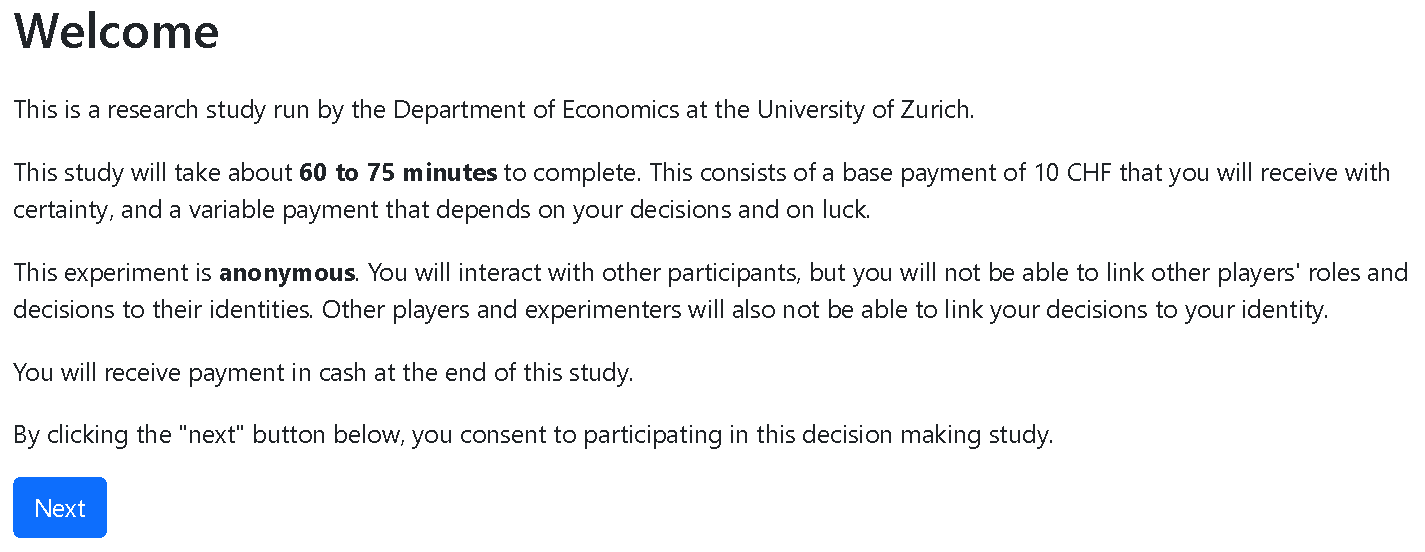
\includegraphics[width=.9\linewidth]{screenshots/welcome.pdf}
    \caption{Welcome screen}
\end{figure}

\begin{figure}[!htb]
    \centering
    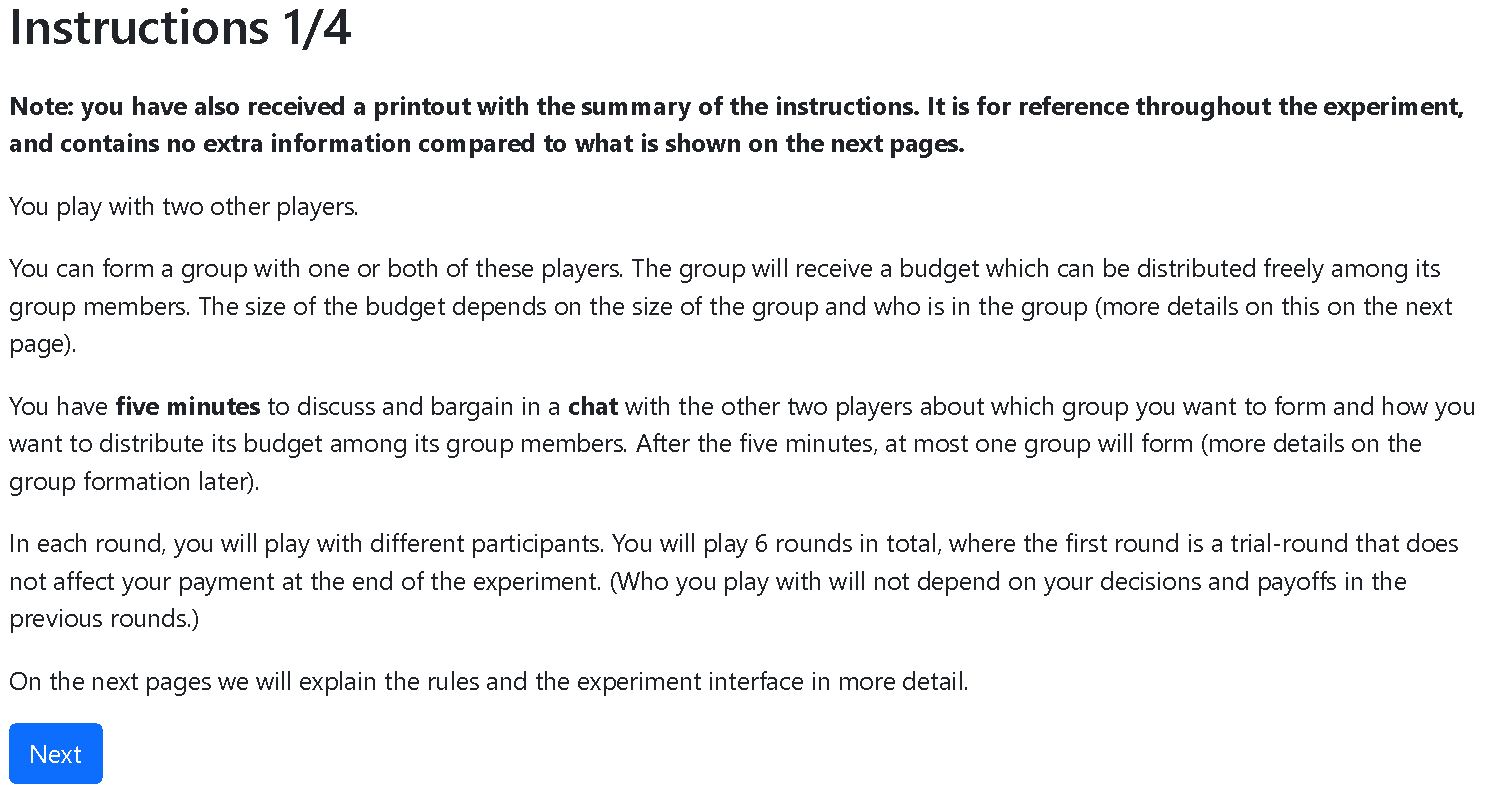
\includegraphics[width=.9\linewidth]{screenshots/instructions_1.pdf}
    \caption{Instructions 1/4: Introduction}
\end{figure}

\begin{figure}[!htb]
    \centering
    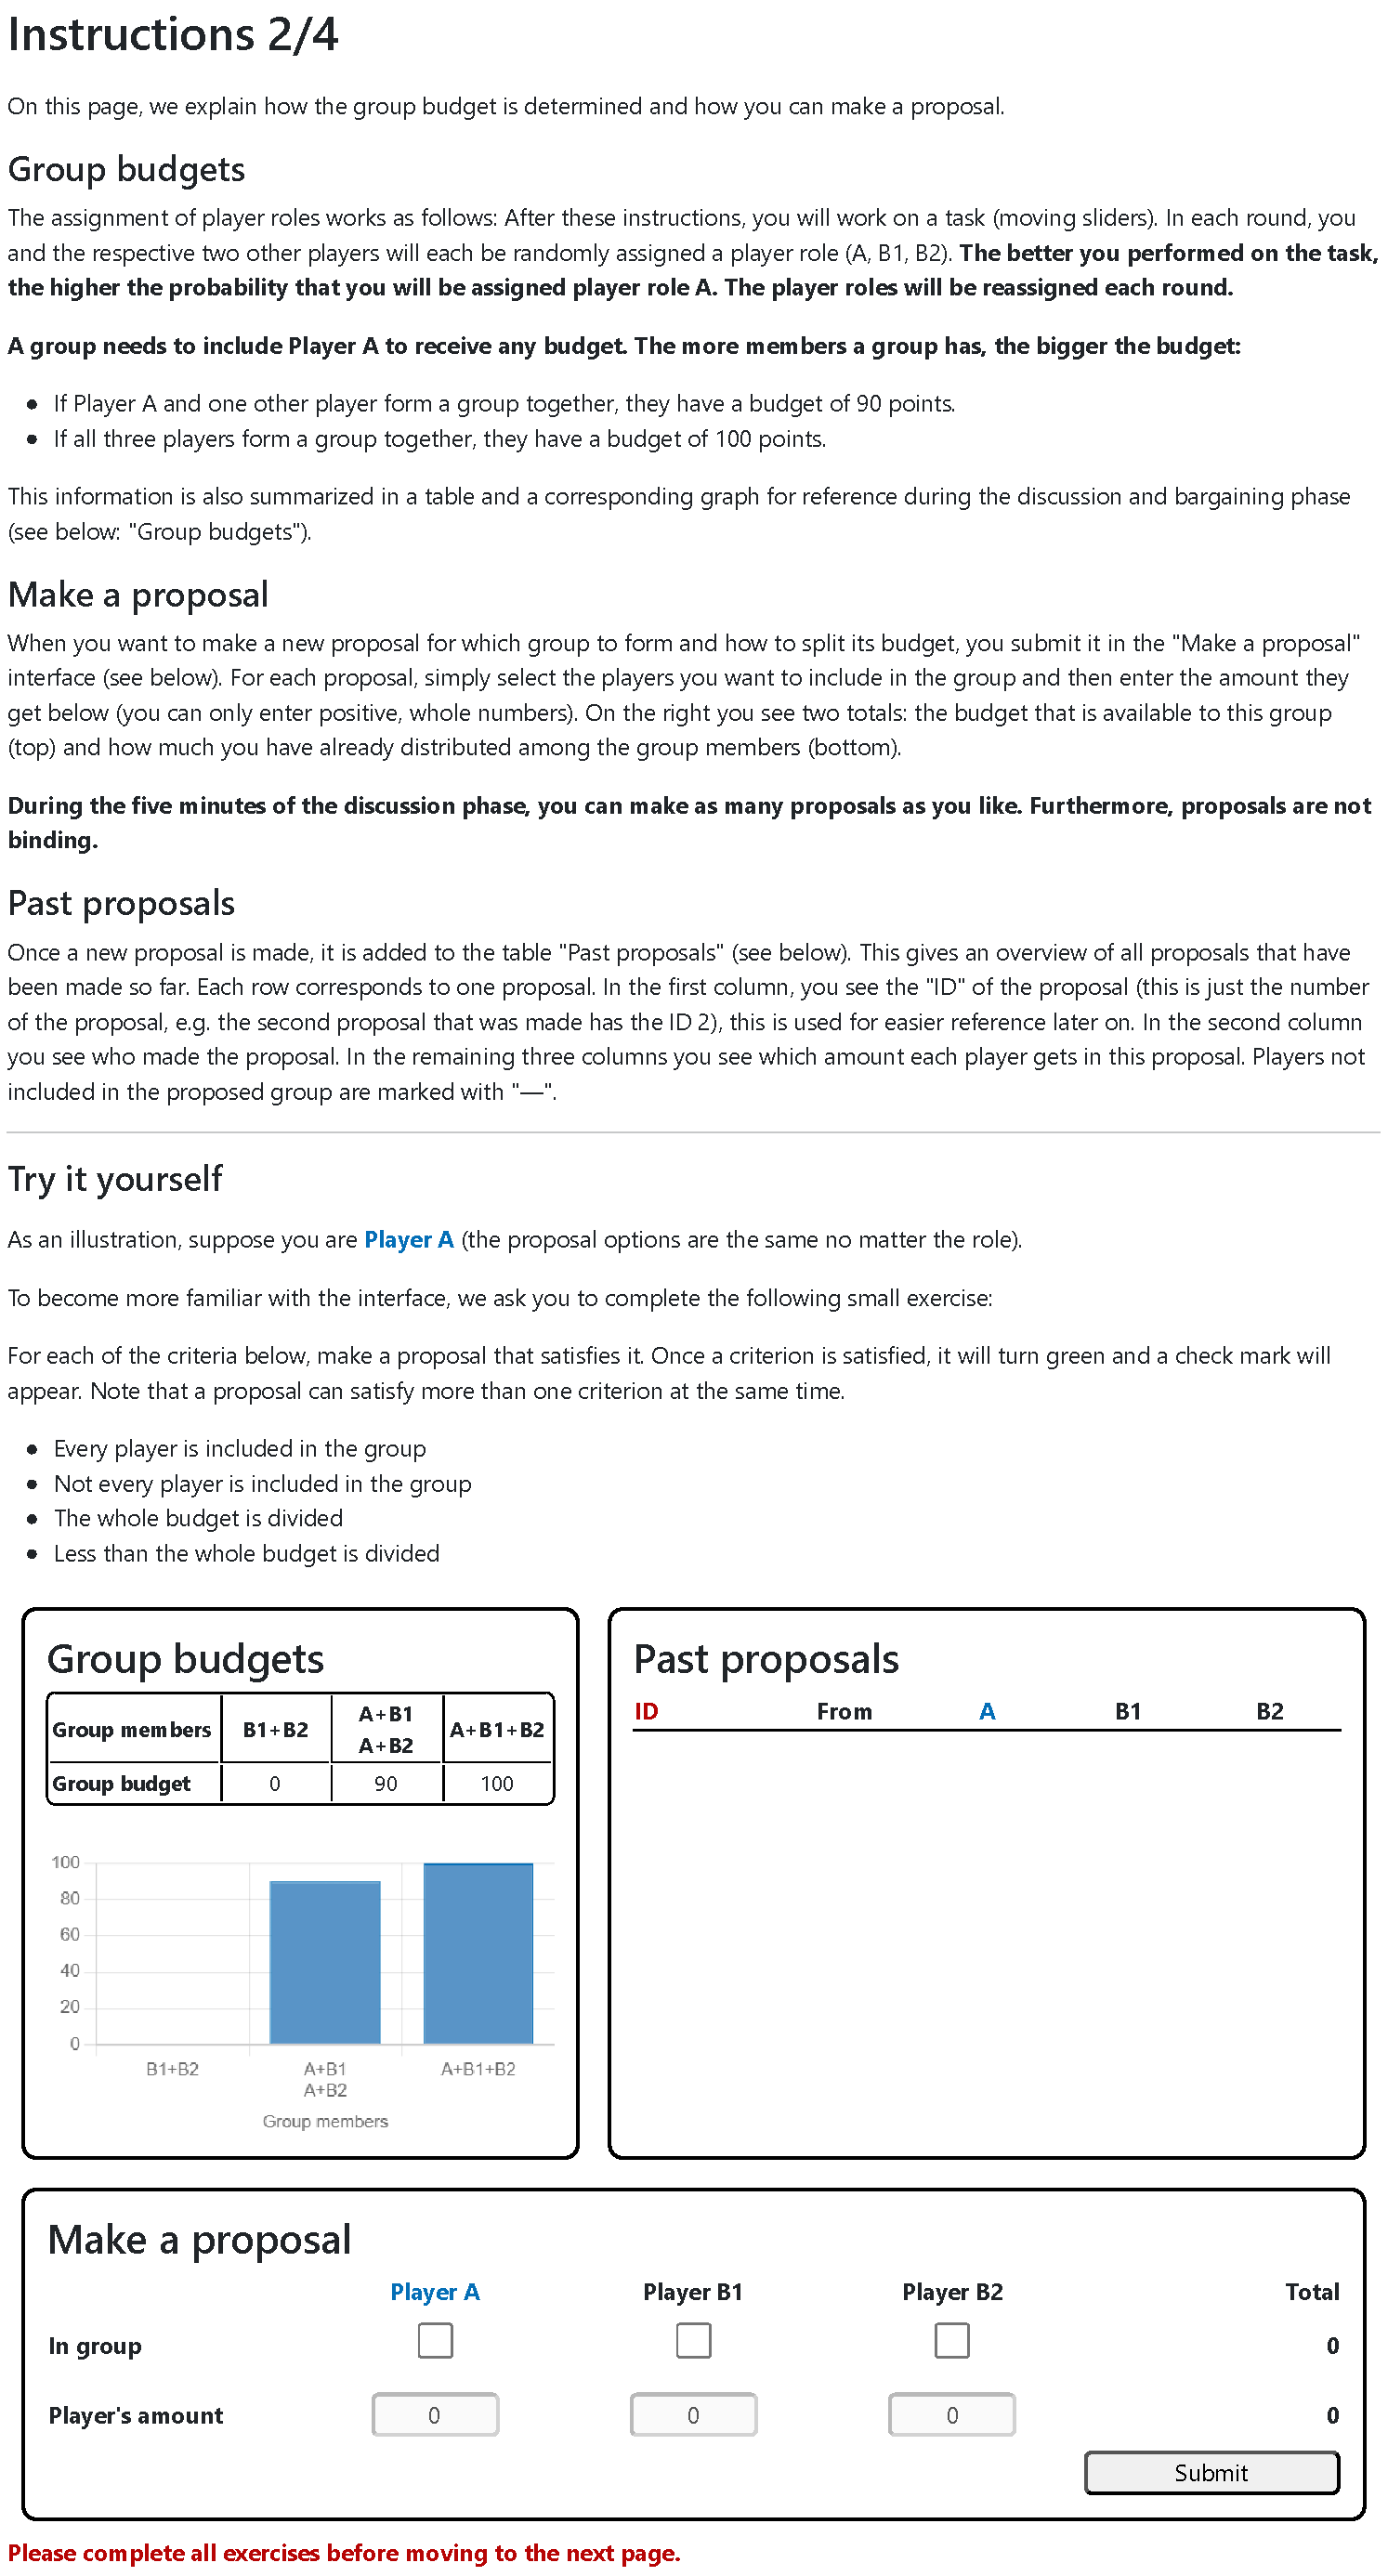
\includegraphics[width=.7\linewidth]{screenshots/instructions_2.pdf}
    \caption{Instructions 2/4: Group budgets}
\end{figure}


\begin{figure}[!htb]
    \centering
    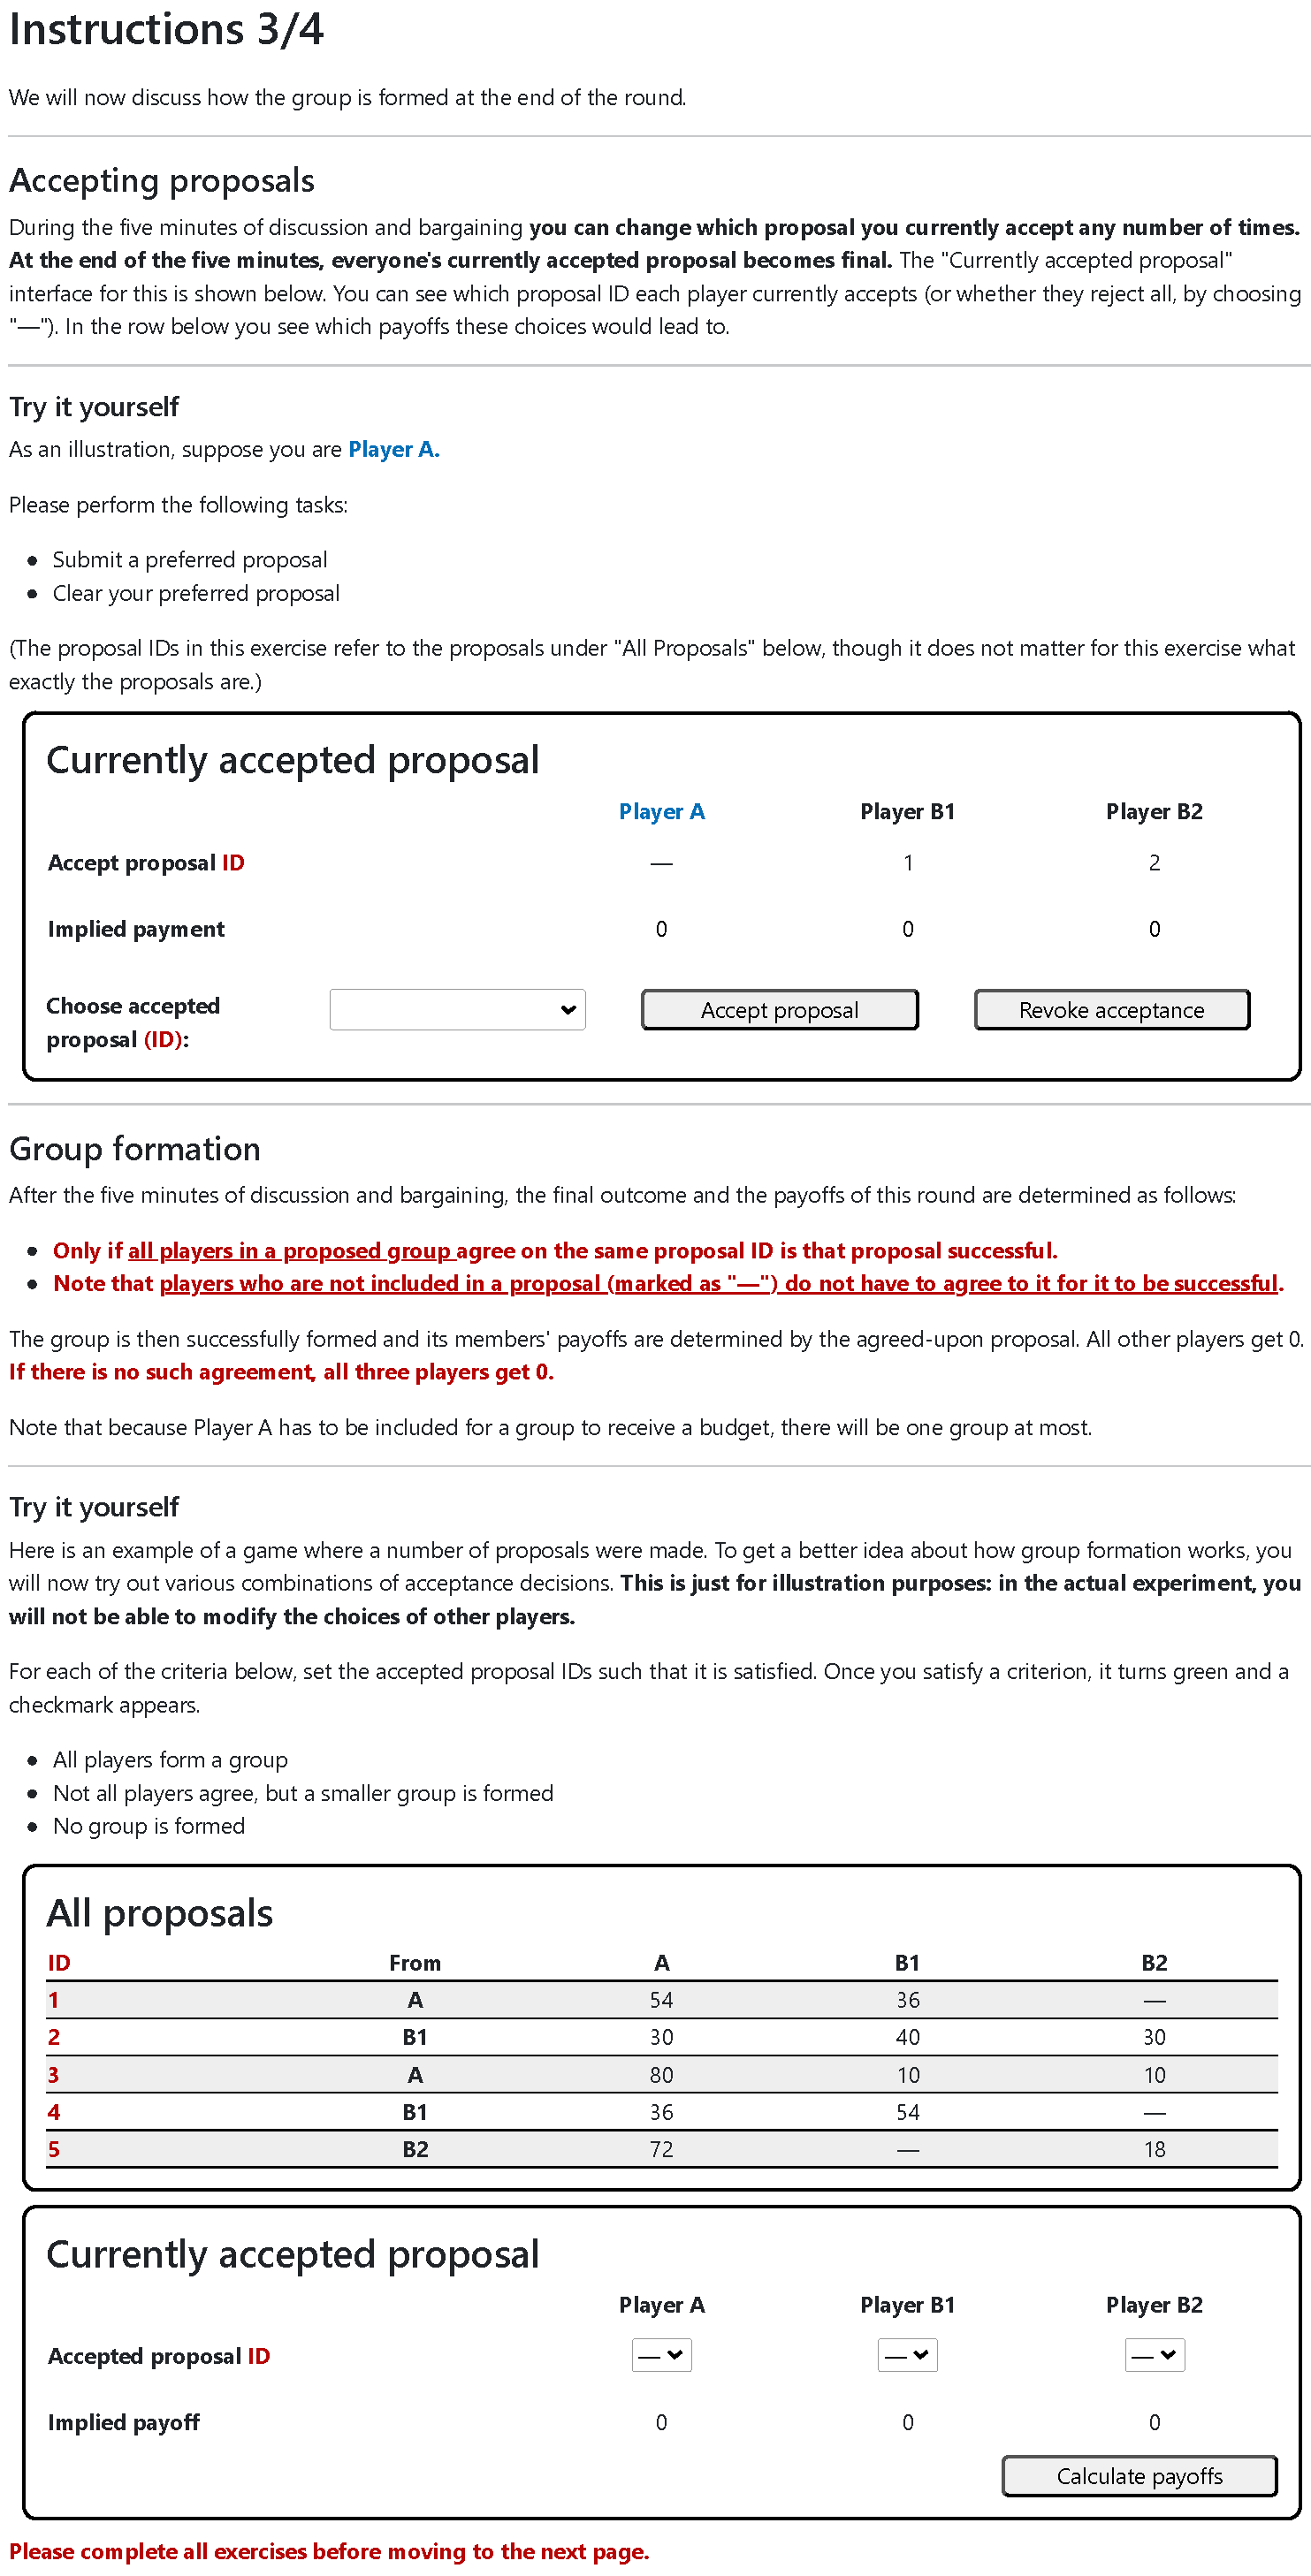
\includegraphics[width=.7\linewidth]{screenshots/instructions_3.pdf}
    \caption{Instructions 3/4: Proposals and group formation}
\end{figure}

\begin{figure}[!htb]
    \centering
    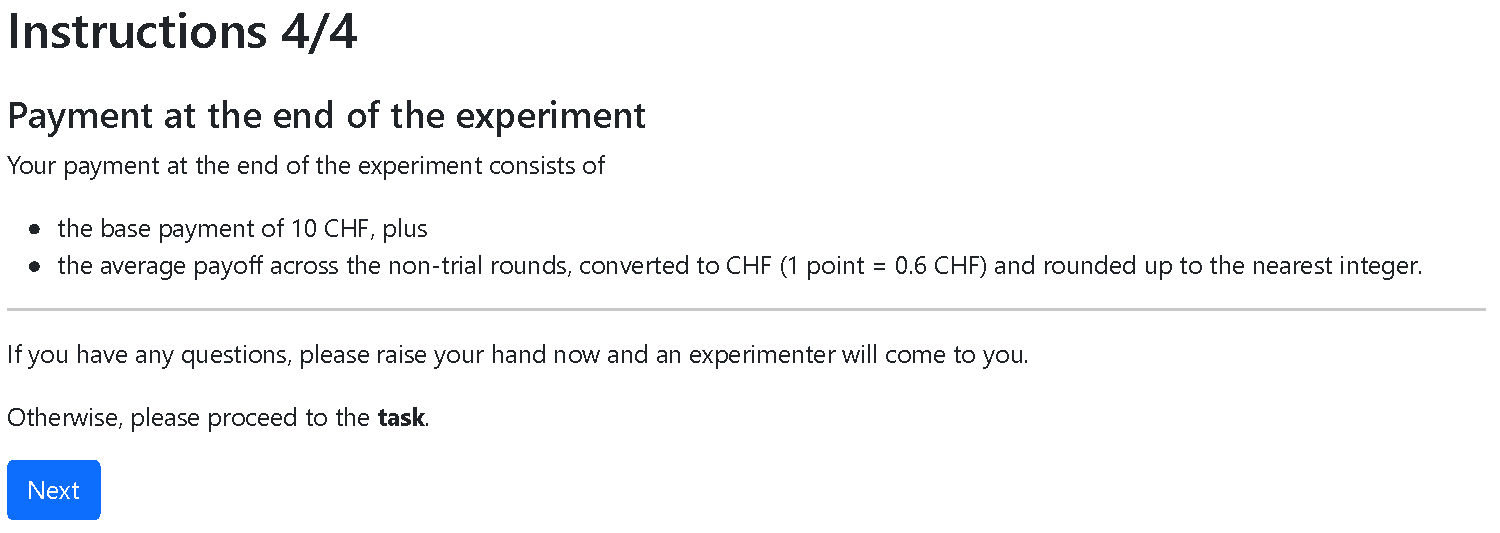
\includegraphics[width=.9\linewidth]{screenshots/instructions_4.pdf}
    \caption{Instructions 4/4: Payment}
\end{figure}


\begin{figure}[!htb]
   \begin{subfigure}[b]{\textwidth}
        \centering
        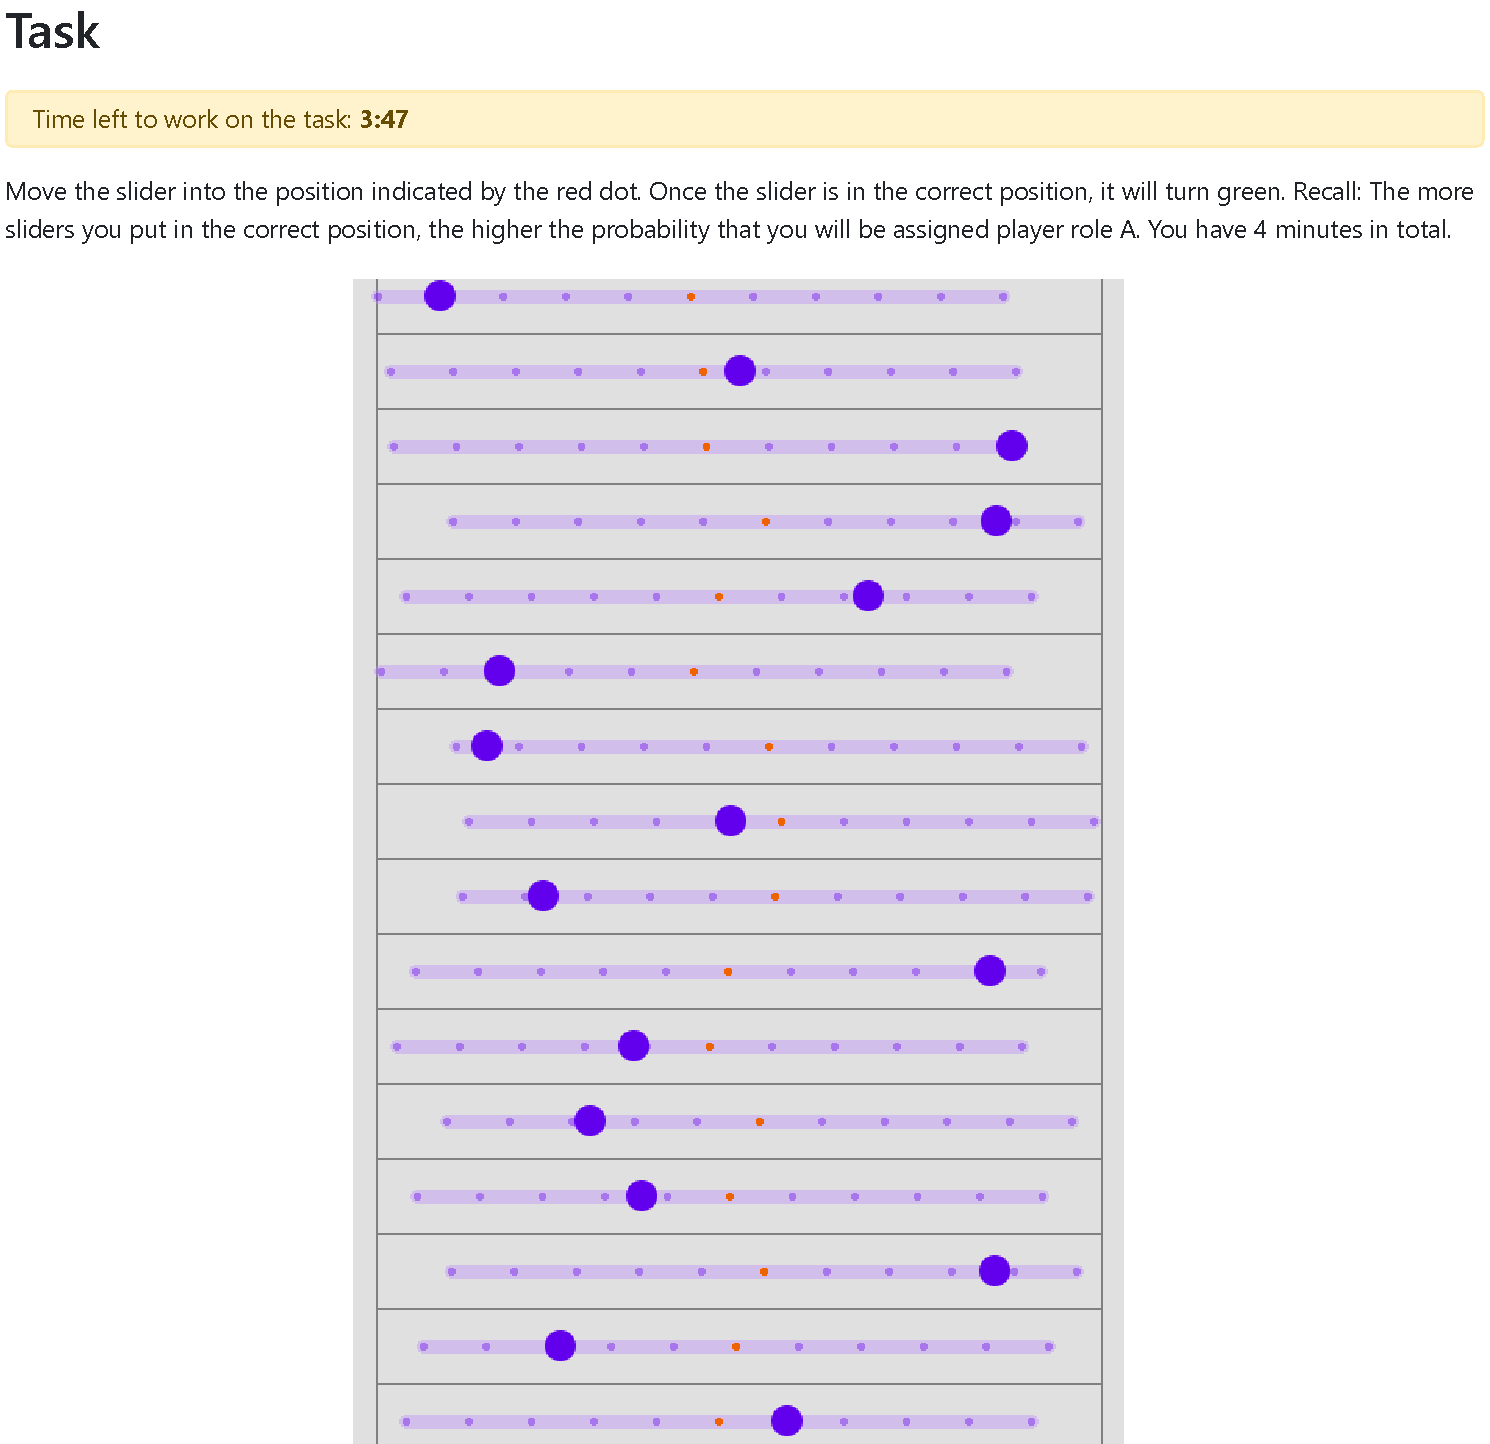
\includegraphics[width=0.9\textwidth]{screenshots/slider.pdf}
    \end{subfigure}
    \par\bigskip
    \begin{subfigure}[b]{\textwidth}
        \centering
        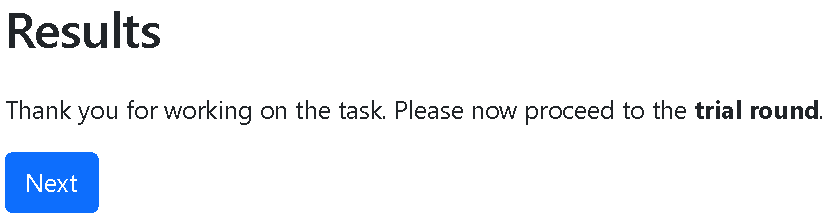
\includegraphics[width=0.5\textwidth]{screenshots/slider_results.pdf}
    \end{subfigure}
    \caption{Slider task. (Note that this screenshot is cropped, there were 150 sliders in total.)}
\end{figure}

\begin{figure}[!htb]
    \centering
    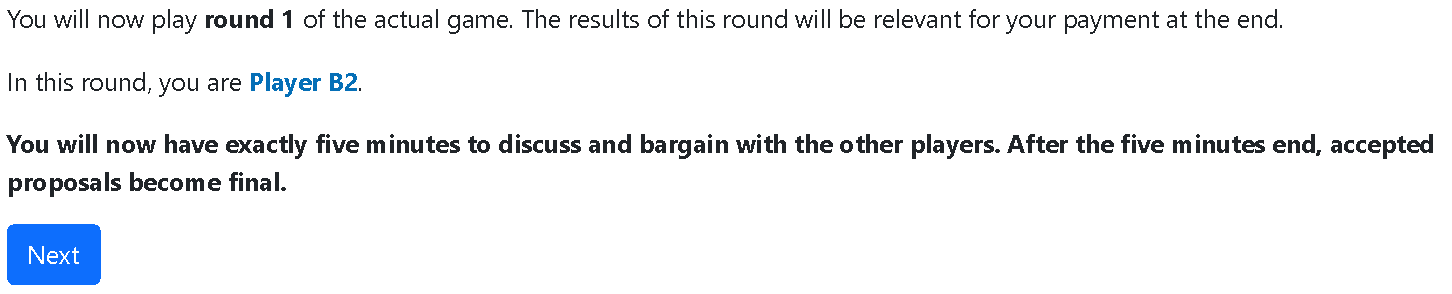
\includegraphics[width=.9\linewidth]{screenshots/info.pdf}
    \caption{Info page before the bargaining round}
\end{figure}

\begin{figure}[!htb]
    \centering
    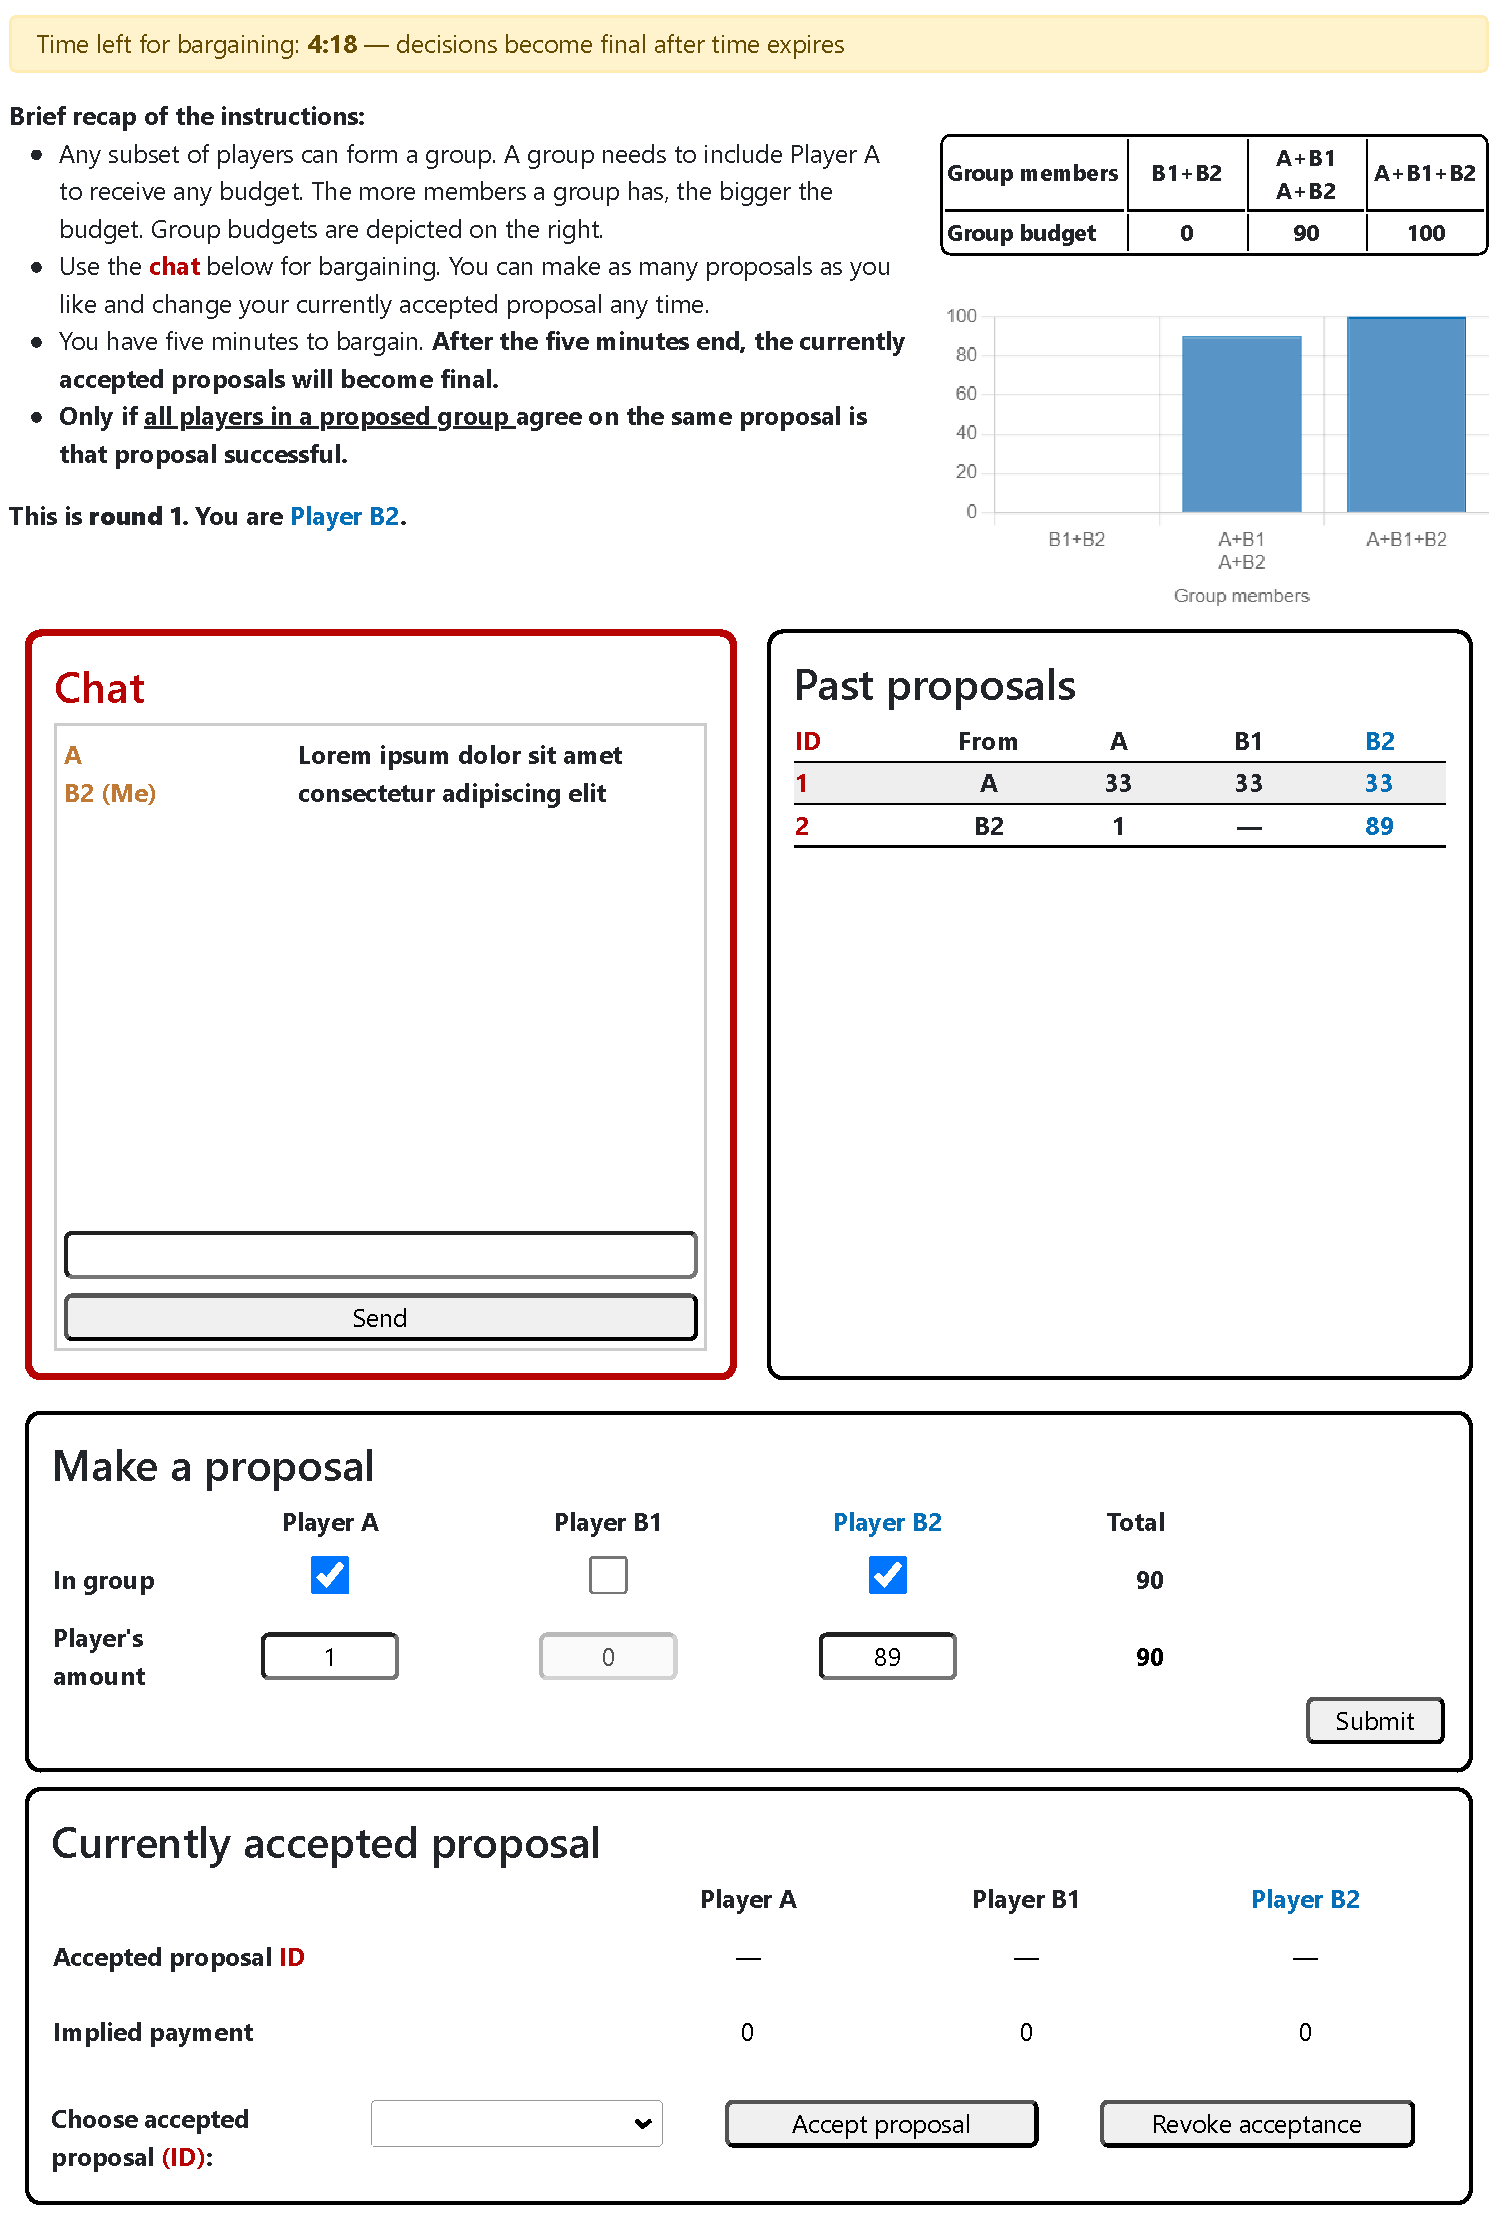
\includegraphics[width=.8\linewidth]{screenshots/bargaining_interface.pdf}
    \caption{Bargaining interface}
    \label{bargaining_interface}
\end{figure}


\section{Chat analysis}

\subsection{Methodology}
\label{sec:gpt_prompt}

To ensure reproducibility as much as possible, the temperature of the GPT-4o model was set to zero. The system prompt we supplied was the following:
\begin{lstlisting}[captionpos=b,caption=System prompt for GPT-4o]
You are going to receive a log containing messages between three players from an economics lab experiment. Players bargained how to split an amount of money. They could additionally use an interface for submitting and accepting proposals. Before the bargaining, players did a slider task and their performance determined their bargaining position.

The log format is the following:
MSG #[MESSAGE_ID] @[PLAYER_NAME]: [MESSAGE]
PROP #[PROPOSAL_ID] @[PLAYER_NAME]: [distribution of the money]
ACC #[ACCEPTANCE_ID] @[PLAYER_NAME]: PROP #[PROPOSAL_ID]
separated by newlines.

Please classify which TOPIC each message (MSG) belongs to. You only have to classify messages, not proposals or acceptances (those latter two are only included for context). The classification should also take into account the context of the message (e.g. when a message is a reply to another).
Each message should be classified into one main and one subtopic. The topics are given in the following nested list:
 - small talk: messages that are not directly related to the experiment
    - greetings and farewells: e.g. saying hello, goodbye, etc.
    - other: e.g. talking about the weather, how to spend the remaining time, etc.
 - bargaining: messages discussing the distribution of the money, making and reacting to proposals, counter-proposals, etc.
    - fairness-based: using arguments based on fairness or justice ideas
    - non-fairness-based: using arguments based on other considerations
 - meta-talk: talking about the experiment itself
    - purpose: discussing what the experimenters are trying to find out
    - rules: discussing and clarifying the rules of the experiment
    - identification: identifying each other, e.g. trying to figure out if players met each other in previous rounds, or identifying information for later

Your response should be of the following format:
#[MESSAGE_ID]: [MAIN_TOPIC], [SUB_TOPIC]
for each message, separated by newlines.
It should look like the contents of a dictionary, but without the surrounding curly braces and apostrophes.
Do not include any other lines, such as code block delimiters or comments.
If there are no rows of type MSG, please respond with NO_MESSAGES without any additional content, such as IDs or comments.
\end{lstlisting}

Then, we supplied the chat, proposal and acceptance history for a given round as the user prompt. An example is given below.
\begin{lstlisting}[captionpos=b,caption=User prompt for GPT-4o]
MSG #1 @A: what are you guys up to?
PROP #1 @B2: A: 34, B1: 33, B2: 33
MSG #2 @A: anyone one split 90 points with me?
MSG #3 @B2: fair play
MSG #4 @B2: propose A
PROP #2 @A: A: 45, B1: 0, B2: 45
ACC #1 @A: PROP #2
MSG #5 @B2: fair i'm down
ACC #2 @B2: PROP #2
MSG #6 @A: i mean if B1 has nothing to say
MSG #7 @A: feel free to offer a better deal :)
MSG #8 @B1: I will not accept it, but i do not think it matters at this point xd
ACC #3 @B1: PROP #0
MSG #9 @A: nope only thing you can do is propose a better deal for me hahah
MSG #10 @A: sorry m8
PROP #3 @B1: A: 46, B1: 44, B2: 0
MSG #11 @A: the power of A
MSG #12 @B1: xdxd no problem
ACC #4 @A: PROP #3
ACC #5 @B1: PROP #3
MSG #13 @A: xD
MSG #14 @A: lets get that game rolling
MSG #15 @A: im sure B2 cannot be happy with that
MSG #16 @B1: hahaha
MSG #17 @B2: :) just wait and see
MSG #18 @A: deal before 10 sek
PROP #4 @B2: A: 50, B1: 0, B2: 40
ACC #6 @B2: PROP #4
ACC #7 @A: PROP #4
\end{lstlisting}

Finally, the model's answer was as follows.
\begin{lstlisting}[captionpos=b,caption=Answer from GPT-4o]
#1: small talk, other
#2: bargaining, non-fairness-based
#3: bargaining, fairness-based
#4: bargaining, non-fairness-based
#5: bargaining, fairness-based
#6: bargaining, non-fairness-based
#7: bargaining, non-fairness-based
#8: bargaining, non-fairness-based
#9: bargaining, non-fairness-based
#10: small talk, other
#11: small talk, other
#12: small talk, other
#13: small talk, other
#14: small talk, other
#15: bargaining, non-fairness-based
#16: small talk, other
#17: small talk, other
#18: bargaining, non-fairness-based
\end{lstlisting}

The results of the categorization of messages is included in the project's git repository along with the raw data.

\subsection{Chat excerpts}
\label{sec:chat_excerpts}

This section contains a number of chat excerpts (including proposals and acceptance decisions) to illustrate some more common themes we observed when reviewing the chat logs. They are presented mostly to give an idea about the kind of textual data we obtained from the experiment.

\begin{figure}[!htb]
    \centering
    \begin{subfigure}[b]{0.42\textwidth}
        \centering
        \includegraphics[width=\linewidth]{out/figures/chat_excerpt-5640,5647-5648,5660-5663.pdf}
        \caption{Treatment $Y=30$: discussing that partial agreement makes no sense}
        \label{fig:chat_stability_y30}
    \end{subfigure}
    \hspace{0.1\textwidth}
    \begin{subfigure}[b]{0.42\textwidth}
        \centering
        \includegraphics[width=\linewidth]{out/figures/chat_excerpt-6846-6847,6849,6851,6853,6855,6857,6859.pdf}
        \caption{Treatment $Y=90$: making the small players compete}
        \label{fig:chat_stability_y90}
    \end{subfigure}
    \caption{Examples of stability-based reasoning from the chat logs. Note, that some messages have been omitted.}
    \label{fig:chat_stability}
\end{figure}

\begin{figure}[!htb]
    \centering
    \begin{subfigure}[b]{0.42\textwidth}
        \centering
        \includegraphics[width=\linewidth]{out/figures/chat_excerpt-7052,7054,7057-7063.pdf}
        \caption{Treatment $Y=90$:, agreeing on almost equal split}
        \label{fig:chat_fairness_equal_split}
    \end{subfigure}
    \hspace{0.1\textwidth}
    \begin{subfigure}[b]{0.42\textwidth}
        \centering
        \includegraphics[width=\linewidth]{out/figures/chat_excerpt-7894-7901,7906.pdf}
        \caption{Treatment $Y=90$: rejecting unequal proposals}
        \label{fig:chat_fairness_reject_small}
    \end{subfigure}
    \caption{Examples of fairness-based reasoning from the chat logs. Note that some messages have been omitted for brevity.}
    \label{fig:chat_fairness}
\end{figure}

\begin{figure}[!htb]
    \centering
    \begin{subfigure}[b]{0.42\textwidth}
        \centering
        \includegraphics[width=\linewidth]{out/figures/chat_excerpt-6508-6509,6511,6513,6524,6527,6528-6529.pdf}
        \caption{Discussing the impact of having the ability to chat with each other}
        \label{fig:chat_meta_chat}
    \end{subfigure}
    \hspace{0.1\textwidth}
    \begin{subfigure}[b]{0.42\textwidth}
        \centering
        \includegraphics[width=\linewidth]{out/figures/chat_excerpt-5501-5508.pdf}
        \caption{Small talk and feedback about the length of the rounds}
        \label{fig:chat_meta_time}
    \end{subfigure}
    \caption{Examples of discussing the experiment from the chat logs. Note that some messages have been omitted for brevity.}
    \label{fig:chat_meta}
\end{figure}

\section{Payoffs by matching group}

\begin{figure}[!htb]
    \centering
    \includegraphics[width=1\linewidth]{out/figures/payoff_matching_group_average_rounds_all.pdf}
    \caption{Average payoff on the matching-group level by role and treatment. (There were six matching groups à six subjects in each treatment.)}
    \label{fig:matching_group}
\end{figure}

\section{Reciprocity concerns}

\begin{figure}[!htb]
    \centering
    \begin{subfigure}[b]{0.49\textwidth}
        \centering
        \includegraphics[width=\textwidth]{out/figures/payoff_average_rounds_[2,3,4,5].pdf}
        \caption{Rounds 1-4}
    \end{subfigure}
    \hfill
    \begin{subfigure}[b]{0.49\textwidth}
        \centering
        \includegraphics[width=\textwidth]{out/figures/payoff_average_rounds_[6].pdf}
        \caption{Round 5}
    \end{subfigure}
    \caption{Average payoffs for each player role by treatment, for the given rounds. Vertical bars denote 95\% confidence intervals for the within-group means.}
    \label{fig:reciprocity}
\end{figure}

A potential concern is that reciprocity is a driver of behavior and leads to more equal payoffs: for example, people might give a non-zero payoff to the dummy player because they expect to be the dummy player in later rounds, or they might agree on outcomes closer to the equal split because they expect to be a small player in later rounds. This is corroborated by the fact that some subjects try to identify each other (\Cref{fig:chat_topics_all}). While a large part of it is due to small talk about topics such as countries of origin or degrees, some subjects tried to agree on code words in order to identify each in later rounds, for example in order to find out if groups were actually reshuffled. Reciprocity, however, would suggest that the behavior in the last round is different from the previous rounds. While we can not exclude that reciprocity is a factor, the comparison of the average payoffs of the last rounds versus all other non-trial rounds does not indicate any substantial difference.

\section{Survey: axioms}

\begin{figure}[!htb]
    \centering
    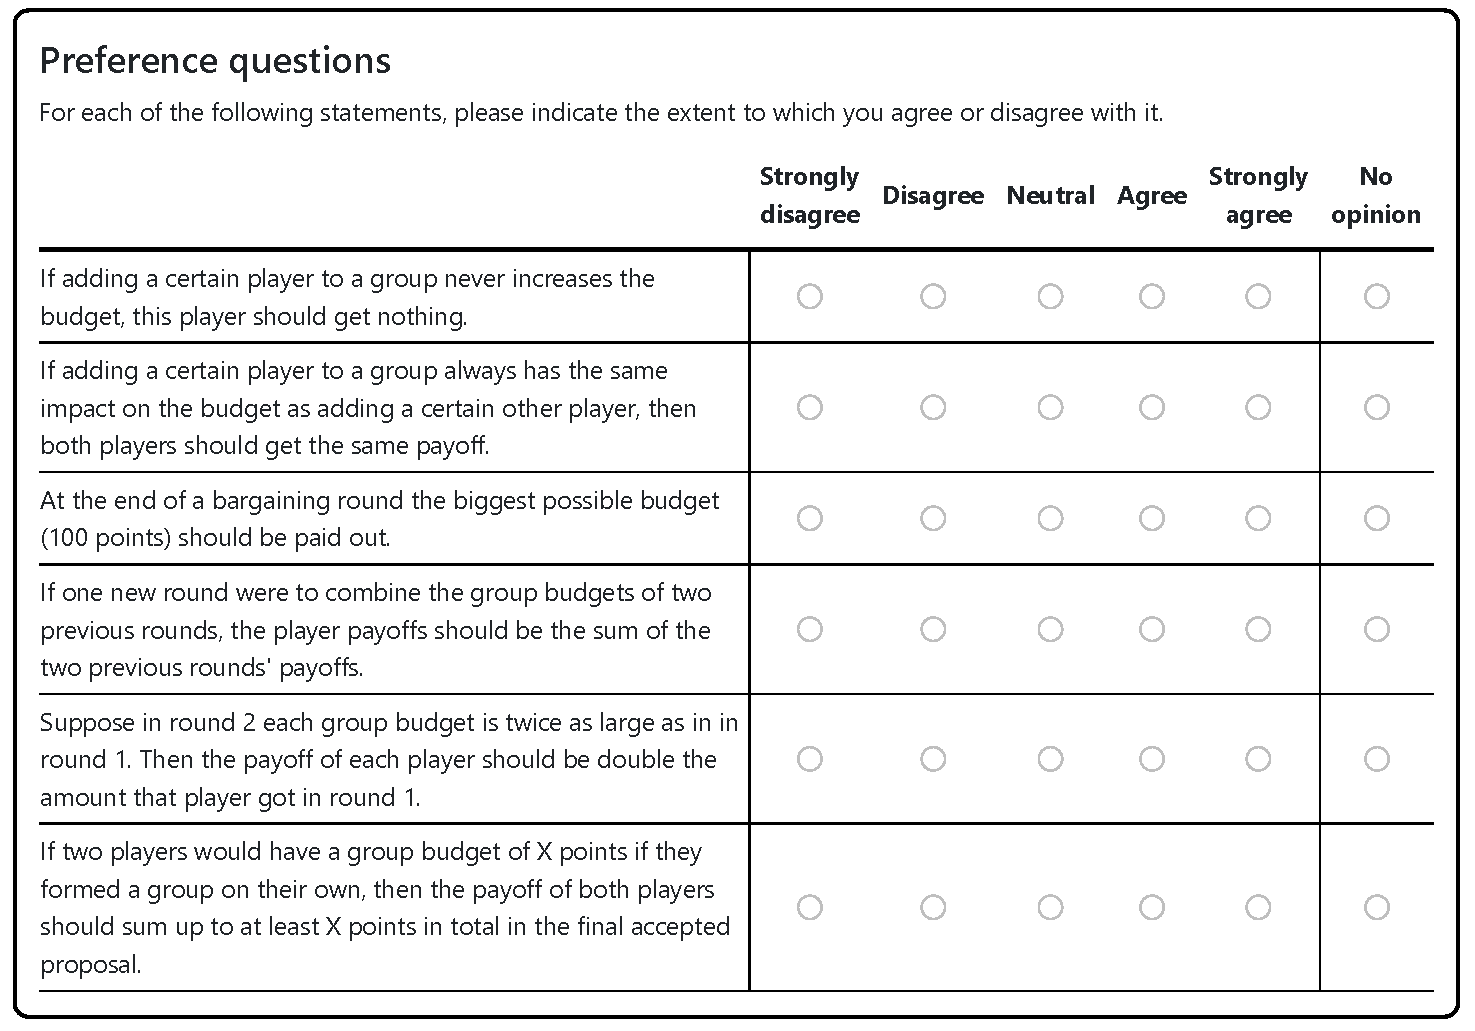
\includegraphics[width=.9\linewidth]{screenshots/survey_axioms.pdf}
    \caption{Survey questions for the axioms}
    \label{fig:survey_axioms_questions}
\end{figure}



\begin{figure}
    \centering
    \includegraphics[width=.99\linewidth]{out/figures/axioms_survey_efficiency.pdf}
    \includegraphics[width=.99\linewidth]{out/figures/axioms_survey_symmetry.pdf}
    \includegraphics[width=.99\linewidth]{out/figures/axioms_survey_linearity_additivity.pdf}
    \includegraphics[width=.99\linewidth]{out/figures/axioms_survey_linearity_HD1.pdf}
    \caption{Survey: empirical support of the axioms}
    \label{fig:axioms_survey_1}
\end{figure}

\begin{figure}
    \ContinuedFloat
    \centering
    \includegraphics[width=.99\linewidth]{out/figures/axioms_survey_dummy_player.pdf}
    \includegraphics[width=.99\linewidth]{out/figures/axioms_survey_stability.pdf}
    \caption{Survey: empirical support of the axioms}
    \label{fig:axioms_survey_2}
\end{figure}


\begin{figure}
    \centering
    \includegraphics[width=1\linewidth]{out/figures/allocations_proposals_by_dummy_player_axiom.pdf}
    \caption{Proposals by agreement with the dummy player axiom.}
    \label{fig:axioms_proposals_dummy_player}
\end{figure}

\begin{figure}
    \centering
    \includegraphics[width=1\linewidth]{out/figures/allocations_proposals_by_symmetry_axiom.pdf}
    \caption{Proposals by agreement with the symmetry axiom.}
    \label{fig:axioms_proposals_symmetry}
\end{figure}

\begin{figure}
    \centering
    \includegraphics[width=1\linewidth]{out/figures/allocations_proposals_by_efficiency_axiom.pdf}
    \caption{Proposals by agreement with the efficiency axiom.}
    \label{fig:axioms_proposals_efficiency}
\end{figure}

\begin{figure}
    \centering
    \includegraphics[width=1\linewidth]{out/figures/allocations_proposals_by_linearity_HD1_axiom.pdf}
    \caption{Proposals by agreement with the linearity (homogeneity of degree 1) axiom.}
    \label{fig:axioms_proposals_linearity_HD1}
\end{figure}

\begin{figure}
    \centering
    \includegraphics[width=1\linewidth]{out/figures/allocations_proposals_by_linearity_additivity_axiom.pdf}
    \caption{Proposals by agreement with the linearity (additivity) axiom.}
    \label{fig:axioms_proposals_linearity_additivity}
\end{figure}

\begin{figure}
    \centering
    \includegraphics[width=1\linewidth]{out/figures/allocations_proposals_by_stability_axiom.pdf}
    \caption{Proposals by agreement with the stability axiom.}
    \label{fig:axioms_proposals_stability}
\end{figure}

\section{Subject sample: Population characteristics} 

\begin{figure}[!h]
    %\centering
    \begin{subfigure}[b]{0.49\textwidth}
        \centering
        \includegraphics[width=\textwidth]{out/figures/survey_gender.pdf}
        \caption{Gender composition, by treatment.}
        \label{fig:balance_gender}
    \end{subfigure}
    \hfill
    \begin{subfigure}[b]{0.49\textwidth}
        \centering
        \includegraphics[width=\textwidth]{out/figures/survey_degree.pdf}
        \caption{Degree composition, by treatment.}
        \label{fig:balance_degree}
    \end{subfigure}
    \vfill
    \begin{subfigure}[b]{0.43\textwidth}
         \centering
        \includegraphics[width=\textwidth]{out/figures/survey_age.pdf}
        \caption{Average age, by treatment.}
        \label{fig:balance_age}
    \end{subfigure}
    \label{fig:balance}
\end{figure}

\begin{figure}
    \ContinuedFloat
    \centering
    \begin{subfigure}[b]{\textwidth}
        \centering
        \includegraphics[width=1\textwidth]{out/figures/survey_nationality.pdf}
        \caption{Nationality composition, by treatment.}
        \label{fig:survey_nationality}
    \end{subfigure}
    \caption{Population characteristics of the experiment sample, by treatment.}
    \label{fig:balance_cont}
\end{figure}


\end{document}
